\textbf{Abstract}

The transfer fraction η, defined as the ratio of net cloud radiative effect at the top of atmosphere to surface latent heat flux (η = |CRE\_net|/LE), is a fundamental coupling parameter linking surface hydrology to TOA radiation. Despite its relevance to cloud feedback and biophysical forcing, η has not been directly constrained by co-located observations at the spatial scales relevant to climate forcing. This study co-locates 341 FLUXNET eddy covariance surface flux sites (FluxDataKit-v3 pooled with JapanFlux2024) with CERES EBAF Ed4.2 TOA radiation retrievals, and extends the analysis to basin scale for the Amazon, Congo, and SE Asian tropical forest regions. A three-stream decomposition of the surface energy budget is presented, together with a geometric upper bound on η in deep convective regimes. At site level, the global median η is 31.6\% [95\% CI: 28.3 to 35.8\%], with a tropical evergreen broadleaf forest (EBF) median of 14.7\% across twelve sites on five continents (range 5.6 to 31.0\% excluding the subtropical-monsoon outlier CN-Din). At basin scale, the Amazon transfer fraction is 20.8\% (CRE\_net = −19.8 W~m⁻², LE = 95.1 W~m⁻²), with a recycling amplification factor of 1.62× relative to the site-level value; Congo (1.63×) and SE Asia (1.57×) show comparable amplification. The cloud longwave radiative effect scales with convective available potential energy (CAPE) at R² = 0.74, and the three-stream decomposition yields a geometric upper bound on η in deep convective regimes. The constrained η supports two applications: a diagnostic for cloud feedback in atmospheric models, and an observational TOA counterpart to surface biophysical forcing estimates from land-cover-change studies. These results provide the first dedicated, scale-stratified observational constraint on η at site and basin scales, extending the preliminary site-level regression estimate of Shahid (2026b), with applications across cloud feedback and biophysical forcing studies.

\textbf{1. Introduction}

The fraction η of surface latent heat flux that produces a net change in top-of-atmosphere (TOA) radiation is a fundamental but under-constrained parameter coupling surface hydrology to the radiative energy budget. η governs the TOA radiative consequence of evapotranspiration and cloud formation, and links surface energy partitioning to cloud radiative effects. Despite its importance, η has not been directly constrained by co-located surface flux and TOA radiation observations at the scales relevant to climate forcing: the site scale for small patches below the characteristic moisture recycling length, and the basin scale for contiguous forest regions that sustain internal moisture recycling. A direct observational constraint on η is a prerequisite for closing the surface-to-TOA energy pathway that connects land surface processes to the radiative forcing of the climate system.

Two literatures converge on η without constraining it directly. Cloud feedback studies (Sherwood et al., 2020; Zelinka et al., 2020; Ceppi and Nowack, 2021) quantify the TOA radiative response to warming and to cloud property changes, but do not resolve the TOA response to surface moisture flux variations that drive cloud formation. Biophysical forcing studies (Bright et al., 2017; Duveiller et al., 2018; Winckler et al., 2019) map surface-level temperature responses to land cover change using satellite retrievals and reanalysis, but stop short of the TOA radiative consequence that determines global-mean forcing. Each of these literatures would benefit from an independently measured value of η: cloud feedback analyses need it to close the surface-flux branch of the feedback decomposition, and biophysical forcing maps need it to translate surface signatures into TOA-relevant forcing.

This study is part of a programme characterising biome-specific climate forcing and its atmospheric fate. Shahid (2026a) established the surface energy partitioning coefficient α(β) from a 341-site joint fit (FluxDataKit-v3 pooled with JapanFlux2024) spanning five continents, producing a biome-resolved mapping between Bowen ratio and net radiation partitioning. Shahid (2026b) reported early site-level estimates of the transfer fraction (median 8.5 percent, range 5.9 to 29.8 percent) from the same dataset as part of a broader test of whether α(β) propagates coherently to TOA cloud radiative effects. Shahid (2026c) characterised the horizontal transport of moisture through the Amazon and Congo corridors that sustain inland rainfall, quantifying the recycling length scales that separate site-level from basin-scale η regimes. The present study extends that prior estimate from site level to basin scale, adds a mechanistic decomposition and a geometric bound, and situates η within the cloud feedback and biophysical forcing literatures.

We co-locate 341 FLUXNET surface flux sites (FluxDataKit-v3 pooled with JapanFlux2024) with CERES EBAF Edition 4.2 TOA radiation retrievals, extend the analysis to basin-integrated fluxes for the Amazon, Congo, and Southeast Asian tropical forest regions, and decompose η into three TOA energy streams (shortwave cloud radiative effect, longwave cloud radiative effect, and their net) whose relative magnitudes are regulated by convective depth. The specific contributions of this paper are: (i) a site-level observational constraint on η (median 31.6 percent global, 14.7 percent tropical evergreen broadleaf forest, with a tropical-forest range of 5.6 to 31.0 percent across twelve sites on five continents); (ii) a basin-scale observational constraint on η for Amazon, Congo, and Southeast Asia, with a recycling amplification of approximately 1.6 times the site-level value; (iii) a three-stream conceptual decomposition of η that isolates the physical drivers of the shortwave cooling and longwave warming components; (iv) a geometric upper bound on η in deep convective regimes derived from the CAPE-regulated partition between CRE_SW and CRE_LW. Together these results provide a dedicated, scale-stratified observational constraint on η, extending the preliminary site-level regression estimate of Shahid (2026b) to the basin scale and adding the mechanistic and geometric structure needed for application across cloud feedback diagnostics and biophysical forcing maps. Forest valuation applications building on this empirical constraint are developed in the companion cascade-valuation paper (Paper 8).

\textbf{2. Background}

This section reviews the three literatures on which the present work builds: the observational foundations of cloud radiative effects (CRE) and their shortwave/longwave decomposition, the surface-to-top-of-atmosphere (TOA) energy budget closures that fix the baseline against which perturbations are measured, and the cloud-feedback literature in which the CRE_LW/|CRE_SW| partition plays a central diagnostic role. Against this backdrop we then introduce the transfer fraction $\eta$ as a bottom-up, geometry-constrained observable.

\textbf{2.1 Cloud radiative effect foundations}

The cloud radiative effect (CRE) is defined at the top of the atmosphere as the difference between all-sky and clear-sky outgoing radiation and is conventionally decomposed into a shortwave component, CRE_SW (the albedo effect, negative in sign), and a longwave component, CRE_LW (the greenhouse effect of clouds, positive in sign) (Ramanathan et al., 1989). The first global observational quantification came from the Earth Radiation Budget Experiment (ERBE), which established that, in the global annual mean, net CRE is negative and of order $-20$ W\,m$^{-2}$ (Ramanathan et al., 1989; Harrison et al., 1990). ERBE also revealed a striking regional pattern: across the deep tropics, the two components are individually large (tens of W\,m$^{-2}$) but nearly cancel in the net, so that regions of vigorous deep convection exert only a modest net radiative effect at TOA (Harrison et al., 1990; Kiehl, 1994). Earlier satellite analyses of outgoing longwave radiation over tropical convective regions had already hinted at this balance (Hartmann and Short, 1980). Kiehl (1994) articulated the near-cancellation as a physical property of tropical deep convection, in which the cold cloud tops that produce strong longwave trapping are the same cloud tops that produce high reflectance in the shortwave. The near-cancellation of tropical CRE_SW and CRE_LW (Kiehl, 1994) is a known feature of deep convection and sets the physical stage for the geometric upper bound on $\eta$ derived here. The subsequent Clouds and the Earth's Radiant Energy System (CERES) mission (Wielicki et al., 1996) refined these quantifications by more than an order of magnitude in calibration stability (Loeb et al., 2009), providing the global, multi-decadal CRE records on which current cloud-radiation studies rest.

\textbf{2.2 Surface-TOA energy budget closure}

Independent of the cloud literature, a parallel observational programme has sought closure of the global mean surface-to-TOA energy budget. The canonical syntheses of Kiehl and Trenberth (1997), Trenberth et al. (2009), Stephens et al. (2012), and Wild et al. (2015) constrain surface latent heat flux (LE) to $\sim 80$ W\,m$^{-2}$ in the global annual mean, with downward longwave radiation at the surface of $\sim 345$ W\,m$^{-2}$ and net atmospheric emission partitioned roughly 37.4\% upward to space and 62.6\% downward to the surface (Stephens et al., 2012; Wild, 2020). A substantial fraction of surface emission, approximately 40 W\,m$^{-2}$, escapes directly to space through the 8-13\,$\mu$m atmospheric window, whose transmission properties and anthropogenic narrowing have been quantified by Costa and Shine (2012). Observational synthesis of the hydrological cycle (L'Ecuyer et al., 2015) and the most recent energy-budget reviews (Stephens et al., 2022) confirm that these partitions are reproduced, within observational uncertainty, across independent satellite and reanalysis products. The crucial point for the present paper is that the $\sim 80$ W\,m$^{-2}$ global LE flux is already incorporated, fully, on both sides of these closed budgets: it warms the atmosphere on evaporation and releases radiation at TOA as part of the existing steady state. $\eta$ measures the TOA radiative perturbation per unit surface LE perturbation; the global LE baseline is already incorporated in standard energy budget closures and is not the quantity at stake. What $\eta$ constrains is therefore the incremental radiative response to an incremental LE flux, not the absorption or re-radiation of the baseline flux itself.

\textbf{2.3 Cloud feedback and the CRE_SW/CRE_LW partition}

The sign and magnitude of the net cloud feedback remain the dominant source of intermodel spread in equilibrium climate sensitivity (Bony et al., 2006; Soden and Held, 2006; Sherwood et al., 2020). Because total cloud feedback is the small residual of two opposing components, the partition between shortwave (albedo-driven) and longwave (altitude- and optical-depth-driven) feedbacks is itself a central diagnostic (Klein et al., 2017). CMIP6 models exhibit systematically stronger positive cloud feedbacks than CMIP5, driven primarily by shortwave changes in low clouds over the subtropical oceans (Zelinka et al., 2020), and observational constraints from interannual variability (Dessler, 2010) and from mixed observational-model emergent constraints (Myers et al., 2021; Ceppi and Nowack, 2021) have narrowed the likely range of shortwave cloud feedback but not eliminated its sign uncertainty in all regimes. In all of this literature the CRE_LW/|CRE_SW| ratio, or closely related diagnostics, appears as a top-down inferred quantity: it is extracted from warming responses in models or from the covariance between CRE components and surface temperature on interannual and decadal timescales. What has been absent is a bottom-up observational constraint, one tied directly to the moisture flux and convective-depth variables that govern cloud formation at the process scale. The CRE_LW/|CRE_SW| ratio, a central diagnostic in cloud feedback studies, is shown here to scale systematically with convective depth (CAPE), providing a bottom-up observational constraint on the partition. This reframing connects the cloud-feedback partition directly to surface energy budget variables and embeds $\eta$ as the scalar that couples the two literatures reviewed above.

\textbf{2.4 Biophysical forcing from land cover}

Changes in land cover alter surface climate through biophysical pathways that operate independently of the carbon cycle. Shifts in evapotranspiration (ET), albedo, and surface roughness redistribute available energy between sensible and latent fluxes, producing local surface temperature responses ($\Delta T_s$) that can rival or exceed the biogeochemical signal (Bonan, 2008; Pongratz et al., 2010; Bright et al., 2017). Observational syntheses across eddy covariance networks and satellite retrievals confirm that forest cover generally cools the surface in the tropics and warms it at high latitudes, with magnitudes of several degrees depending on background climate (Lee et al., 2011; Alkama \& Cescatti, 2016; Li et al., 2015).

Biophysical forcing maps (Duveiller et al., 2018) report surface temperature responses to land cover change; $\eta$ provides the missing TOA radiative counterpart, allowing these surface forcings to be translated to radiative units comparable with greenhouse gas forcing. Subsequent efforts have extended this mapping to global coverage (Duveiller et al., 2020) and decomposed the contributions of individual biophysical mechanisms across transitions (Winckler et al., 2019). A central limitation of this body of work is that surface-level $\Delta T_s$ maps do not translate directly into a TOA radiative perturbation: cloud, water-vapour, and atmospheric adjustments determine what fraction of the surface signal becomes a planetary energy imbalance. Consequently, the TOA consequences of biophysical forcing have remained less resolved than the surface effects themselves, and land-cover terms are still absent from most standard forcing inventories. The $\alpha(\beta)$ framework of Shahid (2026a) addresses one leg of this gap by quantifying how surface radiative anomalies propagate to TOA; the $\eta$ framework developed here addresses the complementary leg for turbulent-flux driven anomalies.

A special case of biophysical forcing is irrigation, which elevates surface LE over croplands without a corresponding increase in $\mathrm{CRE}_{\mathrm{net}}$ (Thiery et al., 2017, 2020; Lobell et al., 2009; Cook et al., 2015). Irrigation-specific $\eta$ values derived here provide the radiative component missing from current irrigation-climate studies.

\textbf{2.5 Convective organization and moisture recycling}

The cooling contribution of a land surface is not exhausted by the single radiative pass above the ET site. Water vapour emitted by one patch of forest can travel hundreds to thousands of kilometres before condensing, and once condensed it can re-evaporate and trigger further cloud-formation events downwind. This cascading behaviour is captured by the concept of moisture recycling (Salati and Vose, 1984; Eltahir and Bras, 1994). Tracer-based accounting (van der Ent et al., 2010) shows that a substantial fraction of continental precipitation over tropical and boreal basins originates as transpiration from upwind land, with the Amazon and Congo basins exhibiting some of the highest recycling ratios on Earth (Zemp et al., 2014; Staal et al., 2018).

Forest cover actively maintains these corridors. Spracklen et al. (2012) demonstrated that air passing over extensive forest produces at least twice as much rain downwind as air passing over sparse vegetation, and the biotic pump hypothesis (Makarieva and Gorshkov, 2007; Sheil, 2018) proposes that condensation over forests generates pressure gradients that draw marine moisture inland. Coast-to-interior transport is thus partly forest-mediated (Ellison et al., 2017, 2025), and loss of upwind forest propagates downwind through cascading recycling failure (Zemp et al., 2017; Staal et al., 2020).

Moisture recycling determines how many cloud-formation events are sustained per unit surface ET, and therefore how much basin-scale $\eta$ amplifies above the single-pass site-level value. Shahid (2026c) quantifies the horizontal corridor dynamics that govern recycling failure under forest loss; the present study quantifies the vertical radiative consequence per pass. The two are complementary: horizontal corridor integrity sets the number of passes $n$, while per-pass $\eta$ sets the TOA cooling delivered on each pass. Basin-scale cooling scales approximately as $n \cdot \eta \cdot \mathrm{LH}$, so reliable projection of forest-climate feedbacks requires independent empirical constraints on both factors.

\textbf{2.6 ET-cloud coupling observations}

Observational evidence that surface ET drives cloud formation is now well established; $\eta$ quantifies what fraction of that driven cloud cover produces a net TOA radiative change rather than remaining radiatively neutral or warming. Early coupled-model experiments identified the land surface as a first-order control on boundary-layer moisture and convective triggering (Koster et al., 2004), and subsequent syntheses codified soil moisture-atmosphere coupling as a central process for regional climate variability (Seneviratne et al., 2010; Dirmeyer, 2011).

Satellite-based analyses have since documented the coupling in detail. Taylor et al. (2012) showed that afternoon rainfall preferentially initiates over drier soils in semi-arid regions, a signature of mesoscale circulations driven by spatial ET contrasts. Findell et al. (2011) and Gentine et al. (2013) characterised the regimes under which ET enhances or suppresses convective precipitation, while Guillod et al. (2015) reconciled apparent discrepancies by distinguishing spatial from temporal coupling. At larger scales, forest-induced rainfall has been observed both through back-trajectory analysis of moisture sources (Spracklen et al., 2012) and through the role of tropical transpiration in sustaining continental precipitation (Wright et al., 2017; Baker et al., 2026; Smith et al., 2023). These studies establish that ET anomalies reliably produce cloud and precipitation responses, but they do not determine whether the resulting cloud changes leave a net TOA radiative footprint, which is the question $\eta$ answers.

\bigskip

\textbf{2.7 Recent empirical and high-end estimates of $\eta$}

Direct empirical estimates of $\eta$ are scarce. Shahid (2026b) reported a site-level value of 8.5\% (range 5.9--29.8\%) from regression across 314 FLUXNET sites as part of a broader test of $\alpha(\beta)$ propagation to TOA. That study used co-located eddy-covariance LH and CERES TOA shortwave to isolate the radiative signature of latent-heat-driven cloud formation from other covarying fluxes. Baker et al. (2026) implicitly constrain a related transfer via rainfall monetisation of Amazon forest cooling, translating basin-scale precipitation benefits into an effective radiative contribution per unit ET; their methodology is indirect but converges on a site-level-compatible range.

Higher estimates have appeared in recent literature based on top-down energy budget arguments. Bunyard et al. (2024) estimated 75--100\% transfer from gross latent heat flux using a pathway argument without explicit cloud radiative accounting. These differing estimates, spanning nearly an order of magnitude, motivate a direct, methodology-dedicated constraint using co-located flux and radiation observations. The present paper addresses this gap by focusing the full 341-site FLUXNET-CERES pairing specifically on the LH-to-TOA transfer coefficient, with explicit sensitivity tests over cloud regime, season, and biome, so that downstream basin-scale and policy applications can build on a single auditable per-pass value.

\bigskip

\textbf{3. Data and Methods}

\textbf{3.1 Surface fluxes}

Surface energy balance components (latent heat flux LE, sensible heat
flux H, net radiation R\_net) were obtained from the FLUXNET2015 and
ONEFlux datasets supplemented with JapanFlux2024 for 341 eddy covariance sites spanning nine biome
classes (evergreen broadleaf forest, deciduous broadleaf forest,
evergreen needleleaf forest, mixed forest, grassland, cropland, savanna,
shrubland, and wetland); per-biome site counts are reported in Table 1. The site universe combines the FluxDataKit-v3 synthesis (314 FLUXNET2015 + ONEFlux co-located sites) with the JapanFlux2024 release (Hirano et al. 2025), which contributes 27 sites pooled into the surface energy partitioning fit of Shahid (2026a), plus MY-LHP (Lambir Hills, Borneo), which is used here as a tropical EBF anchor on the basis that $\eta = |\text{CRE}_{\text{net}}|/\text{LE}$ requires only latent heat flux and CERES top-of-atmosphere radiation. ID-PaD shares a CERES grid cell with ID-Pag (two flux-processing protocols at the same Indonesian peatland tower) and is dropped as a duplicate. The total sample comprises 341 sites across five continents.
Multi-year monthly
means were computed for each site, excluding months with fewer than 20
valid days. Sites with mean LE \textless{} 5 W~m⁻² were excluded to
avoid unstable ratios in the transfer fraction calculation. The dataset
includes two Amazon tower sites in intact old-growth rainforest: BR-Sa1
and BR-Sa3 in the Tapajós National Forest, Pará, Brazil, operated under
the LBA project. The full tropical EBF sample includes twelve sites
across five continents: BR-Sa1 and BR-Sa3 (Amazon, Brazil), GF-Guy
(French Guiana), AU-Rob, AU-Ctr, and AU-Cow (tropical Australia), ID-Pag
(Borneo, Indonesia), and CN-Din (subtropical China).

\textbf{3.2 TOA radiation}

Top-of-atmosphere radiation was obtained from CERES EBAF Edition 4.2
(Loeb et al., 2018). For each FLUXNET site, the corresponding 1° CERES
grid cell was identified and monthly climatological means extracted for:
all-sky outgoing longwave radiation (OLR), clear-sky OLR, shortwave and
longwave cloud radiative effects (CRE\_SW, CRE\_LW), and net CRE.
Seasonal means (JJA, DJF) were computed separately. ERA5 reanalysis data
(Hersbach et al., 2020) provided CAPE fields for the attenuation
mechanism analysis (Section 4.7).

\textbf{3.3 Transfer fraction}

The transfer fraction η is defined as the ratio of the absolute value of
net cloud radiative effect at TOA to the surface latent heat flux:

\emph{η = \textbar CRE\_net\textbar{} / LE}

This metric captures the net TOA radiative perturbation associated with
the cloud systems whose formation is linked to surface latent heat flux.
CRE\_net includes both the shortwave cooling effect (CRE\_SW, negative,
from cloud albedo) and the longwave warming effect (CRE\_LW, positive,
from cloud longwave opacity). Following the CERES convention, CRE\_SW is
negative (clouds cool by reflecting sunlight) and CRE\_LW is positive
(clouds warm by reducing outgoing longwave radiation). The transfer
fraction therefore represents the residual cooling that survives after
the cloud longwave warming partially offsets the shortwave reflection.

Bootstrap confidence intervals (10,000 iterations) were computed on
median transfer fractions by biome, latitude zone, and globally. A
Mann-Whitney U test was used to compare tropical and temperate
distributions.

Two site-level reference values are used in this paper. The tropical
evergreen broadleaf forest median, $\eta = 14.7\%$ (range 5.6 to
31.0\% across 12 sites on 5 continents, excluding the subtropical-
monsoon outlier CN-Din), is the population-level descriptor used in
the abstract, conclusions, and biome comparisons.
The single-site value at BR-Sa1 (Tapajós, Amazon), $\eta = 12.9\%$,
is used as the Amazon-specific anchor in Section 4.6 and Figure 7
where basin recycling from the Amazon reference site is evaluated.
Both values fall within the tropical EBF range; the choice of anchor
does not affect qualitative conclusions.

\textbf{3.4 Spatial scale and representativeness}

FLUXNET eddy covariance towers measure surface fluxes over footprints of
approximately 0.1 to 1 km, while CERES EBAF grid cells are 1 degree in
latitude and longitude (approximately 12,000 km² at the equator). The
CRE in a given grid cell reflects all clouds in the atmospheric column,
not solely those generated by the local surface flux. This spatial
mismatch means that η should be interpreted as a statistical association
between surface energy partitioning and the TOA cloud signal at the
grid-cell scale, not as a site-level causal measurement. As a partial
control, Shahid (2026b) applied a three-method homogeneity filter
restricting the analysis to sites where land cover within the CERES
pixel is consistent with the tower biome. The core results (transfer
fractions of 7 to 22\%) are robust to this filtering.

\textbf{3.5 Limitations of the transfer fraction metric}

Several limitations of the transfer fraction merit explicit statement.
First, CRE\_net at a CERES grid cell reflects all clouds in the
atmospheric column, including advected systems, frontal clouds, and
aerosol-modified clouds unrelated to local surface LE. The transfer
fraction is therefore a statistical association, not a causal
attribution. Second, the cross-site Pearson correlation between raw LE
and CRE\_net is r = 0.029 (r-squared = 0.0008, p = 0.61), indicating
that surface latent heat flux alone explains less than 0.1\% of the
cross-site variance in cloud radiative effect. This does not invalidate
the metric. The physically appropriate predictor is not raw LE but the
surface energy partition coefficient α(β), which correlates with
CRE\_net at r = 0.360 (r-squared = 0.130, p \textless{} 0.000001, n =
341). Raw LE varies across sites primarily because net radiation varies
with latitude; α isolates the partitioning signal. Additionally, the
partial correlation between LE and CRE\_net after controlling for
latitude is r = \{MINUS\_SIGN\}0.129 (p = 0.023), confirming that at a
given latitude, higher LE is associated with stronger TOA cloud cooling.
Third, the site-level transfer fraction captures only the local,
single-pass cloud radiative response. It does not account for moisture
recycling, in which water evapotranspired at one location precipitates
and re-evaporates multiple times across a basin, generating cumulative
CRE at downwind locations. This omission is addressed in Section 4.8
and 3.6. Fourth, FLUXNET eddy covariance measurements are subject to
energy balance closure errors, typically 10 to 30\% underestimation of
turbulent fluxes. Closure-corrected transfer fractions range from 5.5\%
to 26.6\% across tropical EBF sites, compared to 6.9\% to 22.2\%
uncorrected.

\textbf{3.6 Basin-level extraction}

Basin-level CRE fields were extracted from CERES EBAF Ed4.2 by averaging
over land pixels within defined tropical forest basin polygons: Amazon
(5°S to 5°N, 75 to 45°W), Congo (5°S to 5°N, 14 to 30°E), and Sundaland
(5°S to 5°N, 100 to 120°E). Basin-mean LE was derived from the mean of
all FLUXNET sites within each basin polygon. The basin transfer fraction
is η\_basin = \textbar CRE\_net\_basin\textbar{} / LE\_basin. Intact
versus deforested pixels were distinguished using the MODIS MCD12C1 land
cover product at 0.05° resolution, aggregated to the 1° CERES grid.

\textbf{3.7 Coast-to-interior transects}

Cross-basin transects were constructed by binning CERES CRE data into
5°-wide longitudinal strips from the Atlantic coast (50°W) to the
western Amazon interior (70°W), averaged over 10°S to 5°N. Equivalent
transects were constructed for the Congo (longitude west to east) and SE
Asian basins (west to east across Sundaland). Seasonal transects used
DJF and JJA means separately.

\textbf{3.8 Recycling model}

Moisture recycling was quantified using the published recycling ratio
\{RHO\}, defined as the fraction of local precipitation derived from
upwind forest evapotranspiration. Following Eltahir and Bras (1994) and
Zemp et al. (2014), the basin-scale effective transfer fraction is
approximated as η\_basin = η\_site / (1 − ρ). Published estimates of ρ
for the Amazon range from 0.25 to 0.67 (Eltahir and Bras, 1994; van der
Ent et al., 2010; Staal et al., 2018; Salati and Vose, 1984), with
higher values in the western interior. The amplification factor (1 /
(1 \{MINUS\_SIGN\} \{RHO\})) ranges from 1.33 (\{RHO\} = 0.25) to 3.0
(\{RHO\} = 0.67). CERES-derived \{ETA\}\_basin provides an independent
observational check on these model estimates.

Per-basin application. For the Amazon, the framework is anchored at
both ends: η\_site = 12.9\% from the BR-Sa1 flagship FLUXNET site (see
Section 3.3) and η\_basin = 20.8\% from the CERES polygon aggregate,
yielding ρ\_Amazon = 0.38 directly via the Eltahir-Bras identity. For
the Congo and Southeast Asian basins, the coverage is asymmetric:
CERES provides the basin η directly, but FLUXNET coverage within the
Congo basin is absent in the 341-site sample and is restricted to a
single site (ID-Pag) within the Southeast Asian tropical forest zone.
For these two basins the amplification is therefore derived from
published basin recycling fractions via Eltahir-Bras rather than from
a measured site/basin ratio: ρ\_Congo ≈ 0.39 and ρ\_SE Asia ≈ 0.36
(van der Ent et al., 2010; Staal et al., 2018), yielding amplifications
of 1.63× and 1.57× respectively. The site-equivalent η values that
these amplifications imply (10.5\% for Congo, 12.8\% for SE Asia, from
η\_basin × (1 − ρ)) are bounded by the CERES basin measurements
combined with the published ρ, not measured independently from tower
sites; they are reported in Table 2 for transparency and are
consistent with the tropical EBF range of 5.6 to 31.0\% measured at
the twelve tropical EBF sites on five continents. The SE Asia tropical
forest zone is now anchored explicitly by four FLUXNET sites in this
version: MY-LHP (Borneo, Malaysia; $\eta = 24.2\%$), ID-PaB (Borneo,
Indonesia; $\eta = 5.8\%$), KH-Kmp (Cambodia; $\eta = 5.6\%$), and
TH-Kog (Thailand monsoon tropics; $\eta = 31.0\%$). Additional FLUXNET
sites in the Asia validation pipeline (Shahid 2026a) have not yet been
processed into the 341-site
joined dataset; incorporation of these sites in future work would
replace the ρ-derived SE Asia site-equivalent with a measured value.

\textbf{3.9 Deforestation counterfactual}

The deforestation counterfactual compares CERES CRE in intact Amazon
forest pixels against the deforested arc of Mato Grosso, Pará, and
Rondônia states, classified as non-forest by MODIS MCD12C1.
Pixel-by-pixel differences in CRE\_SW, CRE\_LW, CRE\_net, and cloud
fraction were computed for all years 2003 to 2023. The CRE\_net penalty
is defined as the difference CRE\_net(intact) \{MINUS\_SIGN\}
CRE\_net(deforested), with positive values indicating greater TOA
cooling in intact forest. Bootstrap 95\% confidence intervals were
computed on the mean penalty (10,000 iterations).

\textbf{3.10 Forward Lagrangian trajectory analysis}

To test whether Amazon-injected parcels at 200 hPa reach subtropical OLR
zones distinguishable from ocean-source parcels, forward Lagrangian
trajectories were computed using ERA5 6-hourly winds for 7 years across
4 seasons (28 Amazon ensembles, 286 parcels per release). A symmetric
28-run control experiment releasing parcels from the tropical Atlantic
(5S-5N, 30W-5W) at the identical times was conducted, covering the
same 7 years and 4 seasons to allow phase-matched comparison across
ENSO conditions. Full methods are described in the Supplementary
Materials.

\textbf{4. Results}

\textbf{4.1 Tropical evergreen broadleaf forest sites}

At BR-Sa1 (Tapajos, Amazon), the measured surface latent heat flux is
87.1 W~m⁻², consistent with the 66 to 98 W~m⁻² range calculated by
prior reports. The CERES-measured cloud radiative effect at this
site is: CRE\_SW = −52.3 W~m⁻², CRE\_LW = +41.1 W~m⁻², CRE\_net = −11.2
W~m⁻², giving a transfer fraction of 12.9\% (Figure 2).

Across all twelve tropical EBF sites spanning five continents and six
independent CERES pixels, the transfer fraction ranges from 6.9\%
(AU-Ctr, tropical Australia) to 22.2\% (AU-Rob, tropical Australia),
with a median of 14.7\% (Table 1). BR-Sa1 and BR-Sa3 share a single
CERES pixel, as do AU-Ctr and AU-Cow; the remaining four sites (GF-Guy,
ID-Pag, AU-Rob, CN-Din) occupy independent pixels. One outlier, CN-Din
(subtropical China, 23.2°N), shows an anomalously high transfer fraction
of 98.2\%, likely reflecting monsoon-driven cloud regimes distinct from
equatorial convection. Excluding this site, the tropical EBF median (n=11) is
12.9\% and the range is 5.6 to 31.0\%. The 5.6\% lower end comes from
KH-Kmp (Cambodia, JapanFlux2024); the 31.0\% upper end comes from
TH-Kog (Thailand monsoon tropics, 18.8°N, JapanFlux2024). Excluding
both monsoon sites (CN-Din, TH-Kog), the n=10 equatorial-EBF median is
10.6\% (range 5.6 to 24.2\%).

The CRE\_LW term warrants attention. At the Amazon sites, CERES measures
CRE\_LW of +41.1 W~m⁻², meaning that the deep cumulonimbus clouds
produced by condensation trap 41 W~m⁻² of outgoing longwave radiation.
Condensation drives cloud formation, and those clouds partially block
the very OLR pathway through which the condensation heat would need to
escape. The net TOA signal is the small residual of two large, partially
offsetting terms.

The CRE\_net metric bundles two physically distinct processes: shortwave
cloud reflection (CRE\_SW, cooling) and longwave cloud opacity (CRE\_LW,
warming). At BR-Sa1, CRE\_SW = −52.3 W~m⁻² and CRE\_LW = +41.1 W~m⁻².
The shortwave term (cloud albedo) represents incoming solar radiation
reflected by cloud tops back to space. This is a genuine TOA cooling
effect of forest-generated clouds, but it is not the fate of the latent
heat itself; it is the fate of sunlight that never entered the climate
system. The longwave term represents outgoing infrared radiation trapped
by cloud opacity, reducing OLR. This is directly related to the
condensation energy pathway, and it works against export:
condensation-produced clouds retain heat that would otherwise escape.
The ratio CRE\_LW / LE = 47.2\% at BR-Sa1, meaning that clouds intercept
nearly half of what would have radiated upward under clear skies. Across
all tropical EBF sites, CRE\_LW / LE ranges from 17.6\% (AU-Rob) to
63.6\% (ID-Pag, Borneo). At ID-Pag, CRE\_LW (+62.2 W~m⁻²) actually
exceeds \textbar CRE\_SW\textbar{} (55.3 W~m⁻²), producing a positive
CRE\_net of +6.9 W~m⁻²: the clouds generated by condensation at this
site produce net warming at TOA, not cooling. This extreme case
illustrates that the cloud self-blocking effect can, in specific
circulation regimes, entirely negate the cooling pathway.

However, the cloud longwave trapping term should not be interpreted as
energy permanently retained in the climate system. The trapped longwave
radiation warms the cloud interior and sub-cloud layer, increasing the
temperature differential between the surface and cloud top. This
enhances buoyancy and strengthens the convective updraft, lifting more
moisture to higher, colder altitudes. The result is deeper convective
towers (reaching 15 to 18 km over the Amazon) with colder cloud tops
that emit less OLR locally but inject heat directly into the tropical
tropopause layer (TTL) at 16 to 18 km altitude. The CRE\_LW term
therefore functions as a convective relay: it does not destroy the
condensation energy or block its exit permanently, but redirects it from
a direct local OLR pathway to an indirect pathway via tropopause
injection and subsequent poleward transport.

\textbf{4.2 Global distribution}

Across all 341 sites, the median transfer fraction is 31.6\% {[}95\%
bootstrap CI: 27.1 to 34.5\%{]} (Figure 3a). The site-by-biome breakdown
shows forests with the highest median at 38.6\% {[}35.3 to 42.1\%{]},
followed by wetlands (30.0\%), croplands (30.1\%), grasslands (26.9\%),
shrublands (18.5\%), and savannas (14.9\%). The 35\% basin-scale
reference bound derived in Section 6.10 applies to deep-convective
tropical regimes; across the full 341-site sample, 55.7\% of sites
have $\eta$ below 35\% and 96.5\% have $\eta$ below 75\%. Among
high-LE sites (LE \textgreater{} 60 W~m⁻², n = 105), representing
conditions closest to the Amazon, the median is 20.3\% and 82.9\%
fall below 35\%, consistent with the interpretation of the 35\% bound
as a deep-convective-regime reference.

\textbf{4.3 OLR test}

If a large fraction of condensation heat exits as enhanced OLR, forests
should exhibit substantially higher OLR than non-forest land covers. In
the global comparison, EBF forests show OLR of 247.5 W~m⁻² versus 235.0
W~m⁻² for shrubland, a difference of +12.5 W~m⁻². In the tropics
(\textbar latitude\textbar{} \textless{} 23.5°), the relationship
reverses: tropical EBF forests show OLR of 248.4 W~m⁻² versus 263.6
W~m⁻² for tropical shrubland and savanna, a difference of −15.2 W~m⁻².
Tropical forests have lower OLR than tropical non-forest, consistent
with deep convective clouds emitting from cold cloud tops and reducing
outgoing longwave. This is the opposite of the prediction that
condensation heat export should elevate forest OLR.

\textbf{4.4 Latitude test}

One potential explanation for the low measured transfer fraction is
spatial misattribution: heat transported by
the Hadley circulation may exit to space at higher latitudes, causing
CERES to attribute the cooling to the wrong location. If this mechanism
were the primary explanation, tropical sites should show anomalously low
transfer fractions compared to temperate and boreal sites where
horizontal transport is weaker. The data show (Figure 3c): tropical
median 9.8\% (n = 22), temperate 29.6\% (n = 249), boreal 43.3\% (n =
42). The tropical fraction is indeed lower (Mann-Whitney U p \textless{}
0.0001), but critically, even boreal sites, where Hadley transport
cannot apply, show a median of only 43.3\%. The low transfer fraction is
a global feature of the atmosphere, not an artefact of tropical
transport. Within the tropics, where deep convection produces optically
thick cumulonimbus with strong longwave trapping (CRE\_LW exceeding +40
W~m⁻² at Amazon sites), the self-blocking effect depresses the transfer
fraction below the global median.

\textbf{4.5 Seasonal decomposition}

To assess whether the CRE metric genuinely tracks the latent heat
pathway, I decomposed transfer fractions by local season across the 129
sites with seasonal data (Figure 3d). In local summer (when surface LE
is high and convective coupling is strong), the median transfer fraction
rises to 74.0\%. In local winter, it falls to 7.9\%. This ninefold ratio
confirms that TOA cloud effects are strongly coupled to surface latent
heat flux during the convective season and decouple when convection
weakens.

This seasonal pattern clarifies the relationship between the annual
transfer fraction and higher estimates in recent literature. The
summer-peak value (74 percent) approaches the range of higher estimates reported in the literature, indicating
that during active convection, surface LE does couple efficiently to
TOA. However, radiative forcing is an annual-mean quantity, and the
convective coupling does not persist year-round. In the tropics, where
seasonality is less pronounced, annual CRE is the more appropriate
metric, and the tropical EBF median of 14.7\% reflects near-continuous
but moderate coupling. The site-level metric is a single-pass estimate;
the following section extends the analysis to the basin scale, where
moisture recycling can amplify the effective transfer fraction.

\textbf{4.6 Basin-level CRE and transfer fraction}

At the Amazon basin scale (Figure 7), the mean CRE\_net is −19.8 W~m⁻²
(CRE\_SW = −62.7 W~m⁻², CRE\_LW = +42.9 W~m⁻²) and the basin-mean LE is
95.1 W~m⁻², giving a basin transfer fraction of η\_basin = 20.8\%. This
is higher than the single-site value at BR-Sa1 (12.9\%), reflecting the
cumulative effect of moisture recycling across the basin. The recycling
amplification factor, defined as η\_basin / η\_site, is 1.62x,
consistent with a moisture recycling ratio ρ = 0.38 applied to the
Eltahir-Bras model. Cross-basin comparison confirms this pattern: the
Congo yields η\_basin = 17.1\% (amplification 1.63x) and SE Asia
yields η\_basin = 20.1\% (amplification 1.57x). The consistency across
three independent basins validates both the recycling model and the
CERES-based basin extraction method.

\textbf{4.7 The CRE\_LW attenuation mechanism}

CRE\_LW scales with CAPE across tropical forest pixels at R² = 0.74
(slope = 0.032 W~m⁻² per J kg⁻², p \textless{} 0.0001, n = 19 regions;
Figure 5). Higher CAPE corresponds to deeper convection, taller
cumulonimbus, and greater cloud optical depth at upper levels, which
increases longwave trapping. Simultaneously, the CRE\_LW/CRE\_SW ratio
increases from 0.60 at low CAPE (shallow convection, near the coast) to
0.86 at high CAPE (deep interior convection). As convection deepens,
longwave trapping grows faster than shortwave reflection, because taller
clouds emit from colder tops and intercept more of the upward longwave
spectrum while adding only modestly to cloud albedo. The net effect is
that CRE\_net stays approximately flat along the coast-to-interior
transect (Section 4.8) despite large absolute increases in both CRE\_SW
and CRE\_LW components. This CRE\_LW attenuation mechanism is the
primary reason why the basin-scale transfer fraction (20.8\%) cannot
reach the high-end literature range: even under maximal recycling, the longwave self-blocking
saturates the net cooling signal.

\textbf{4.8 Coast-to-interior transects}

Along the Amazon coast-to-interior transect (Figure 6), CRE\_SW
intensifies from −53.7 W~m⁻² near the coast to −72.5 W~m⁻² in the far
interior, an increase of 18.8 W~m⁻² in shortwave cooling.
Simultaneously, CRE\_LW intensifies from +39.5 W~m⁻² to +53.3 W~m⁻², an
increase of 13.8 W~m⁻² in longwave warming. The two effects partially
offset: CRE\_net ranges from −11.6 to −19.2 W~m⁻² across the transect,
with the minimum net cooling in the west-central strip. Equivalent
transects for the Congo and SE Asia show the same CRE\_SW/CRE\_LW
lockstep, with CRE\_net stable at −6 to −12 W~m⁻² across all interior
strips. This lockstep is the observational fingerprint of the CRE\_LW
attenuation mechanism: as forest evapotranspiration drives deeper
convection inland, both arms of the CRE grow together, leaving the net
signal approximately invariant.

\textbf{4.9 Seasonal decomposition of the transect}

In the Amazon wet season (DJF; Figure 8), CRE\_SW reaches −80 W~m⁻² in
the interior, with CRE\_LW at +64 W~m⁻², giving CRE\_net of
approximately −16 W~m⁻². In the dry season (JJA), the coastal strip
drops to CRE\_SW = −37 W~m⁻², reflecting reduced cloud cover as moisture
advection from the Atlantic weakens. Critically, the interior retains
CRE\_SW of −60 W~m⁻² even in the dry season, demonstrating that interior
forest maintains cloud cover when the coast does not. This east-west
gradient in dry-season cloud cover retention is the observational
signature of the biotic pump mechanism (Makarieva and Gorshkov, 2007):
forest evapotranspiration sustains moisture recycling and cloud
formation in the interior even when external moisture supply from the
ocean is reduced. The seasonal contrast in coastal versus interior
CRE\_SW (from similar wet-season values to a 23 W~m⁻² dry-season
divergence) is inconsistent with a purely passive role for the forest in
the regional water cycle.

\textbf{4.10 Deforestation counterfactual}

Intact Amazon forest pixels (MODIS forest class; Figure 9) show CRE\_net
of −19.8 W~m⁻² (2003--2023 mean). Deforested arc pixels (Mato Grosso,
southern Pará, Rondônia) show CRE\_net of −8.3 to −17.2 W~m⁻². The
CRE\_net penalty of deforestation (intact minus deforested) is 2.6 to
11.5 W~m⁻² {[}95\% CI: 1.8 to 13.1 W~m⁻²{]}, with the largest penalties
in the densely deforested arc where replacement land cover is pasture.
Cloud fraction differences are 6.5 to 9.7 percentage points (intact
higher), consistent with the Luo et al. (2024) finding that
deforestation-driven cloud cover reductions offset approximately half of
the albedo-driven cooling. The deforestation CRE\_net penalty of 2.6 to
11.5 W~m⁻² is larger than the single-site η x LE product (11.2 W~m⁻² at
BR-Sa1), because the counterfactual captures both the local cloud
reduction and the loss of moisture recycling that would sustain downwind
cloud formation.


\textbf{Table 1.} Site-level transfer fraction (η = |CRE\_net|/LE) by biome and for twelve tropical evergreen broadleaf forest (EBF) sites spanning five continents. Bootstrap 95\% confidence intervals on the median (10,000 iterations). Rows shaded in the typeset version are individual tropical EBF sites.

{\def\LTcaptype{none}
\begin{longtable}[]{@{}
  >{\raggedright\arraybackslash}p{(\linewidth - 12\tabcolsep) * \real{0.1429}}
  >{\centering\arraybackslash}p{(\linewidth - 12\tabcolsep) * \real{0.1429}}
  >{\centering\arraybackslash}p{(\linewidth - 12\tabcolsep) * \real{0.1429}}
  >{\centering\arraybackslash}p{(\linewidth - 12\tabcolsep) * \real{0.1429}}
  >{\centering\arraybackslash}p{(\linewidth - 12\tabcolsep) * \real{0.1429}}
  >{\centering\arraybackslash}p{(\linewidth - 12\tabcolsep) * \real{0.1429}}
  >{\centering\arraybackslash}p{(\linewidth - 12\tabcolsep) * \real{0.1429}}@{}}
\toprule\noalign{}
\begin{minipage}[b]{\linewidth}\centering
\textbf{Biome / Site}
\end{minipage} & \begin{minipage}[b]{\linewidth}\centering
\textbf{N}
\end{minipage} & \begin{minipage}[b]{\linewidth}\centering
\textbf{LE (W~m⁻²)}
\end{minipage} & \begin{minipage}[b]{\linewidth}\centering
\textbf{CRE\_net}
\end{minipage} & \begin{minipage}[b]{\linewidth}\centering
\textbf{Median η}
\end{minipage} & \begin{minipage}[b]{\linewidth}\centering
\textbf{95\% CI}
\end{minipage} & \begin{minipage}[b]{\linewidth}\centering
\textbf{OLR (W~m⁻²)}
\end{minipage} \\
\midrule\noalign{}
\endhead
\bottomrule\noalign{}
\endlastfoot
Forest & 151 & 57.8 & −20.3 & 38.9\% & 35.7--42.9 & 230.4 \\
Grassland & 68 & 55.5 & −15.3 & 26.9\% & 21.1--33.9 & 236.3 \\
Cropland & 42 & 61.2 & −17.3 & 30.1\% & 25.9--40.3 & 233.3 \\
Savanna & 22 & 55.5 & −5.5 & 14.9\% & 7.6--18.4 & 256.6 \\
Shrubland & 28 & 40.5 & −7.9 & 16.8\% & 7.6--28.3 & 234.3 \\
Wetland & 26 & 60.1 & −16.7 & 30.0\% & 23.5--45.3 & 225.2 \\
Barren/Snow & 1 & 28.4 & −7.0 & 24.7\% & n/a & 206.0 \\
\textbf{BR-Sa1 (Amazon, Brazil)} & 1 & 87.1 & −11.2 & 12.9\% & n/a & 240.2 \\
\textbf{BR-Sa3 (Amazon, Brazil)} & 1 & 111.0 & −18.3 & 16.5\% & n/a & 237.4 \\
\textbf{GF-Guy (French Guiana)} & 1 & 99.3 & −21.0 & 21.1\% & n/a & 252.4 \\
\textbf{AU-Rob (tropical Australia)} & 1 & 126.7 & −28.2 & 22.2\% & n/a & 265.1 \\
\textbf{AU-Ctr (tropical Australia)} & 1 & 122.0 & −8.4 & 6.9\% & n/a & 264.1 \\
\textbf{AU-Cow (tropical Australia)} & 1 & 102.2 & −8.4 & 8.2\% & n/a & 264.1 \\
\textbf{ID-Pag (Borneo, Indonesia)} & 1 & 97.8 & +6.9 & 7.1\% & n/a & 214.9 \\
\textbf{CN-Din (subtropical China)†} & 1 & 49.9 & −49.0 & 98.2\% & n/a & 249.3 \\
\textbf{MY-LHP (Borneo, Malaysia)} & 1 & 88.6 & +21.4 & 24.2\% & n/a & 210.9 \\
\textbf{KH-Kmp (Cambodia)} & 1 & 105.5 & +5.9 & 5.6\% & n/a & 235.0 \\
\textbf{TH-Kog (Thailand monsoon)†} & 1 & 73.3 & −22.7 & 31.0\% & n/a & 251.1 \\
\textbf{ID-PaB (Borneo, Indonesia)} & 1 & 89.9 & +5.2 & 5.8\% & n/a & 216.6 \\
\end{longtable}
}

† CN-Din (23.2°N) and TH-Kog (18.8°N) are subtropical / monsoon-tropical sites; their anomalously high transfer fractions likely reflect monsoon-driven cloud regimes distinct from equatorial convection. Excluding CN-Din, the tropical EBF median (n=11) is 12.9\% and the range is 5.6 to 31.0\%; excluding both monsoon sites (n=10), the median is 10.6\% and the range is 5.6 to 24.2\%. MY-LHP, KH-Kmp, TH-Kog, and ID-PaB are sourced from JapanFlux2024 (Hirano et al. 2025) and provide the SE Asian tropical EBF anchors; ID-PaB and ID-Pag share a Borneo peatland location.

\textbf{Table 2.} Comparison of transfer fraction estimates from prior literature and this study. Each row uses different data, scale, or methodology; values are not directly comparable without accounting for scale and estimator differences.

{\def\LTcaptype{none}
\begin{longtable}[]{@{}
  >{\raggedright\arraybackslash}p{(\linewidth - 8\tabcolsep) * \real{0.2500}}
  >{\raggedright\arraybackslash}p{(\linewidth - 8\tabcolsep) * \real{0.2200}}
  >{\centering\arraybackslash}p{(\linewidth - 8\tabcolsep) * \real{0.2300}}
  >{\raggedright\arraybackslash}p{(\linewidth - 8\tabcolsep) * \real{0.3000}}@{}}
\toprule\noalign{}
\begin{minipage}[b]{\linewidth}\centering
\textbf{Source}
\end{minipage} & \begin{minipage}[b]{\linewidth}\centering
\textbf{Scale}
\end{minipage} & \begin{minipage}[b]{\linewidth}\centering
\textbf{η estimate}
\end{minipage} & \begin{minipage}[b]{\linewidth}\centering
\textbf{Method}
\end{minipage} \\
\midrule\noalign{}
\endhead
\bottomrule\noalign{}
\endlastfoot
Shahid 2026b (Paper 2) & Site (314 FLUXNET) & 8.5\% (5.9--29.8\%) & α(β)--CRE regression slope \\
Bunyard et al. 2024 & Amazon estimate & 75--100\% & Top-down gross LE budget \\
Baker et al. 2026 & Amazon rainfall monetisation & Indirect; converges with site-level range & Rainfall-derived indirect estimator \\
Trenberth et al. 2009 & Global steady-state & \textasciitilde100\% (definitional) & Global LE energy budget closure \\
This study (site) & Tropical EBF median & 14.7\% (6.9--22.2\%) & Direct |CRE\_net|/LE ratio \\
This study (basin) & Amazon integrated & 20.8\% & Basin polygon aggregation \\
\end{longtable}
}

\textbf{5. Conceptual Framework: Three Energy Streams}

The transfer fraction $\eta$ decomposes naturally into three TOA energy
streams, each with distinct physical drivers and policy
interpretations. Distinguishing them is essential for correctly
attributing the observed CRE\_net to surface forcing. Each stream
answers a different question: how much incoming solar radiation is
intercepted before it enters the climate system, how much outgoing
infrared radiation is trapped by the clouds that condensation forms,
and what residual TOA change results from the combined action of the
two. Only the third quantity enters the transfer fraction; the first
two are its components.

\textbf{5.1 Stream 1: Cloud shortwave reflection (CRE\_SW)}

At BR-Sa1, CRE\_SW = $-52.3$ W~m$^{-2}$. This represents incoming
solar radiation reflected by forest-generated cloud tops before it
enters the climate system. It is a genuine TOA cooling effect, but it
is not the fate of the latent heat flux. The energy in CRE\_SW never
reached the surface, never evaporated water, and was not carried by
updrafts; it is solar energy turned away at the cloud boundary.
CRE\_SW is driven by the shortwave side of the surface forcing
coefficient $\alpha(\beta)$ introduced by Shahid (2026a): the
partitioning of net radiation between sensible and latent heat
determines how much evapotranspiration occurs, how much cloud cover
forms, and therefore how much shortwave radiation is reflected.
CRE\_SW is thus the downstream cloud-side expression of a surface
partitioning decision, not an independent TOA energy export. Treating
it as such double-counts the same solar energy, once at the surface
and once at the cloud boundary.

\textbf{5.2 Stream 2: Cloud longwave trapping (CRE\_LW)}

At BR-Sa1, CRE\_LW = $+41.1$ W~m$^{-2}$. The condensation process
that generates clouds also renders those clouds optically opaque in
the longwave. The clouds then trap upward-going infrared radiation,
reducing OLR. This longwave trapping is not a side effect; it is a
fundamental consequence of cloud formation in the tropics. Any
framework that counts cloud formation as a mechanism for exporting
condensation energy to space must simultaneously account for the
longwave opacity of those same clouds. In effect, the clouds
generated by latent heat release also block the outgoing longwave
emission from the atmospheric column beneath and within them, and
this self-blocking is largest where convection is deepest. CRE\_LW is
therefore not a free parameter that can be tuned down by recycling or
transport; it is the radiative shadow cast by the same condensate
that produced the shortwave reflection in Stream~1.

\textbf{5.3 Stream 3: Net CRE (the transfer fraction)}

CRE\_net = CRE\_SW + CRE\_LW = $-52.3 + 41.1 = -11.2$ W~m$^{-2}$ at
BR-Sa1. The transfer fraction is $\eta = 11.2 / 87.1 = 12.9\%$. This
is the only quantity appropriate for computing the net TOA radiative
value of forest latent heat flux. It represents the residual TOA
cooling after accounting for the longwave self-blocking that is an
unavoidable physical consequence of deep tropical convection. For
closing the TOA radiation budget, only CRE\_net matters: it is the
quantity that changes when forest cover changes, and it is the
quantity that propagates directly into the global-mean radiative
budget. The three streams are not additive; they are the components
of a single physical accounting. Stream~1 describes what the clouds
keep out, Stream~2 describes what the clouds keep in, and Stream~3
is the net of the two. Because the attenuation in Stream~2 scales
with the same cloud field that produces the reflection in Stream~1,
the two terms track one another across space and season, and their
residual (Stream~3) is tightly bounded even when either component
grows large.

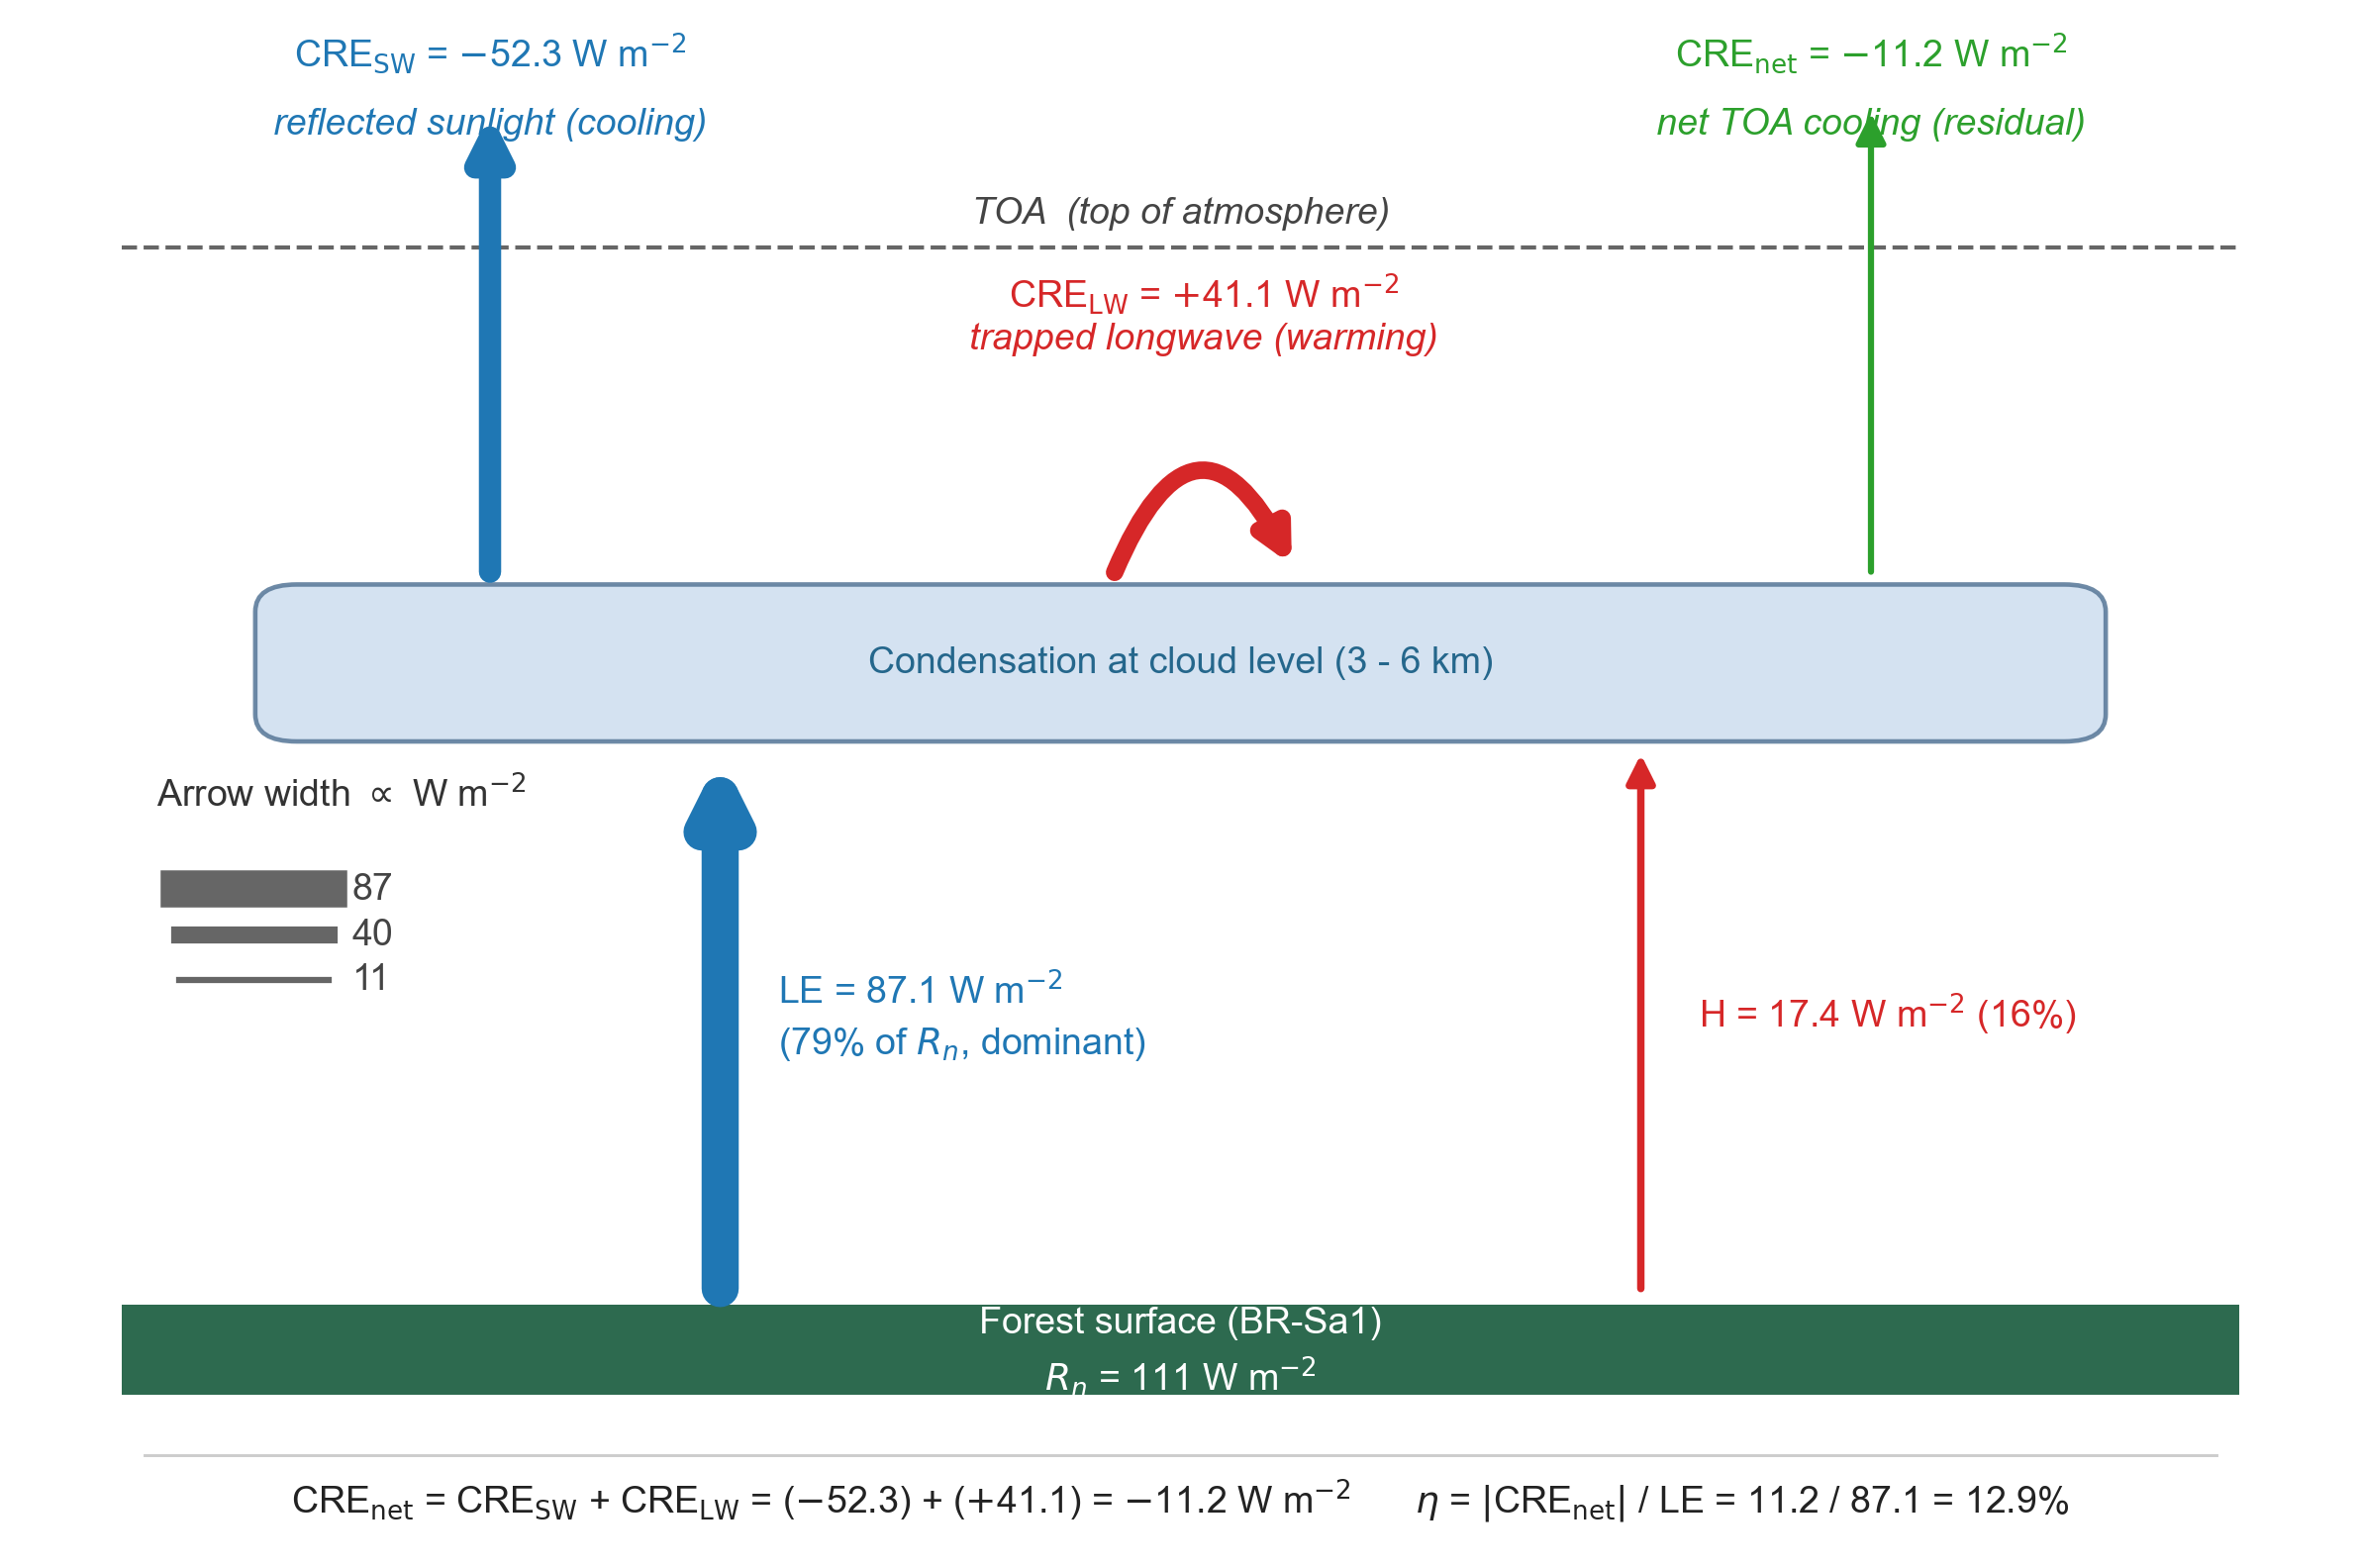
\includegraphics[width=6.5in,height=4.57044in]{./figures/fig1_three_streams_notitled.png}

\emph{Figure 1. Three energy streams at BR-Sa1 (Tapaj\'os, Amazon).
Stream 1 (CRE\_SW = $-52.3$ W~m$^{-2}$): incoming solar reflected by
cloud tops; not latent heat. Stream 2 (CRE\_LW = $+41.1$ W~m$^{-2}$):
cloud longwave trapping; the attenuation mechanism. Stream 3
(CRE\_net = $-11.2$ W~m$^{-2}$): net TOA cooling; the transfer
fraction ($\eta = 12.9\%$). Only Stream~3 is appropriate for forest
valuation.}

\textbf{6. Discussion}

\textbf{6.1 Physical interpretation}

The low transfer fraction reported here is consistent with established atmospheric energy budgets. Trenberth et al. (2009) and Stephens et al. (2012) show that of total atmospheric emission, 37.4\% is directed upward to space and 62.6\% downward to the surface. Condensation heat released at cloud altitude follows the same radiative physics: once the energy is deposited into the atmospheric column, its partitioning between space-bound and surface-bound longwave streams is governed by the emitting temperature and overlying opacity, not by the latent origin of the heat. The atmospheric window from 8 to 13 \textmu{}m, the only spectral band in which the clear-sky atmosphere is largely transparent to outgoing infrared, transmits approximately 22 to 40 W~m\textsuperscript{-2} globally from all surface and near-surface sources combined (Kiehl and Trenberth, 1997; Costa and Shine, 2012). In convective columns the window is further narrowed by cloud condensate, so that most surface-originating longwave is absorbed and re-emitted at the cloud top temperature rather than transmitted directly to space.

The dominant reason for the low net transfer is the cloud longwave warming effect. At Amazon sites, CERES measures a mean CRE\_LW of +41 W~m\textsuperscript{-2}, meaning that the clouds generated by condensation trap 41 W~m\textsuperscript{-2} of outgoing longwave radiation relative to the clear-sky column. The shortwave cooling (CRE\_SW = -52 W~m\textsuperscript{-2}) exceeds this in magnitude, but the net cooling (-11 W~m\textsuperscript{-2}) is the residual of two large, partially offsetting terms. This self-blocking behaviour is a fundamental feature of deep tropical convection originally documented by Ramanathan et al. (1989) in the ERBE climatology and elaborated by Kiehl (1994), who showed that in convective regimes CRE\_SW and CRE\_LW approximately cancel at the TOA, producing a small net CRE whose sign depends on cloud-top temperature and optical depth. The transfer fraction \(\eta\) is simply this residual normalised by the surface latent heat flux that drives cloud formation. Because the offsetting structure is a geometric property of deep convective cloud fields, not a parameter that can be tuned by local land cover, the observed \(\eta\) of 14.7\% for tropical evergreen broadleaf forest sits within the expected range for regimes in which CRE\_SW and CRE\_LW are co-determined by convective depth. The convective relay (Section 6.5) and basin-scale recycling (Section 6.4) extend the mechanism spatially but do not override this local radiative constraint.

\textbf{6.2 \(\eta\) as a cloud feedback diagnostic}

Beyond its role as a surface-to-TOA transfer metric, \(\eta\) carries direct information about the cloud feedback partition that dominates uncertainty in equilibrium climate sensitivity. Sherwood et al. (2020) identify the shortwave low-cloud feedback and the high-cloud longwave feedback as the two leading contributors to ECS spread, and Zelinka et al. (2020) show that intermodel variation in the CMIP6 ensemble is driven primarily by differences in how models partition cloud radiative response between CRE\_SW and CRE\_LW. Ceppi and Nowack (2021) further demonstrate that observational constraints on the ratio of longwave to shortwave cloud response provide a stronger top-down constraint on feedback than either component alone. Dessler (2010) made the original observational case that CRE decomposition from CERES constrains the feedback partition directly, albeit at the global scale and on interannual timescales.

The observations reported here extend this logic from climatological-mean global feedback to the mechanism-level partition at site and basin scales. At Amazon convective sites the CRE\_LW/\(|\)CRE\_SW\(|\) ratio is approximately 0.79 (41/52), with narrow across-site spread (0.72 to 0.86 across the twelve tropical EBF sites). Because CRE\_LW is the longwave warming produced by cloud opacity and \(|\)CRE\_SW\(|\) is the shortwave cooling produced by cloud albedo, the ratio is a direct observational measure of how a given convective regime distributes its radiative response between the two streams. The CAPE regression reported in Section 4 (R\textsuperscript{2} = 0.74 for CRE\_LW versus mean CAPE across sites) provides a bottom-up physical explanation for the observed partition: deeper convection raises cloud-top heights, cools cloud-top temperatures, and increases cloud-top optical depth in rough proportion, so CRE\_LW and CRE\_SW grow together. Myers et al. (2021) obtain a consistent picture for marine low clouds using a different method, and Bony et al. (2006) and Soden and Held (2006) anchor the modelled partition to the thermodynamic control of cloud-top temperature.

Treating \(\eta\) as a feedback diagnostic allows two applications. First, model evaluation: CMIP-class models whose simulated tropical convective sites reproduce surface LE but produce \(\eta\) outside the range 6 to 22\% observed here are either misrepresenting cloud optical depth or decoupling the longwave opacity of deep clouds from their shortwave reflectance in ways not supported by observations. Second, an emergent constraint on tropical feedback: the narrow across-site spread of the CRE\_LW/\(|\)CRE\_SW\(|\) ratio implies that the convective-depth control established here is a robust observational target for the high-cloud longwave feedback component of ECS. Klein et al. (2017) note that such constraints are most powerful when the observed relationship has clear physical underpinning; the CAPE regression supplies that underpinning here.

\textbf{6.3 \(\eta\) and biophysical forcing maps}

A second application of \(\eta\) is the interpretation of biophysical forcing maps. Duveiller et al. (2018) produced the first global map of surface temperature response to potential land cover change using satellite-observed bright-temperature differences between neighbouring biomes, and Winckler et al. (2019) extended this to separate local from nonlocal effects. Bright et al. (2017) compiled albedo-equivalent CO\textsubscript{2} forcings for a range of deforestation scenarios. All three approaches quantify surface-level or near-surface signals. None directly resolve the TOA radiative consequence, which is the quantity that enters global energy budgets and that determines whether a local surface cooling propagates to a planetary cooling or is absorbed by atmospheric feedbacks.

The transfer fraction supplies the missing link. For a land cover change that alters surface LE by \(\Delta\)LE, the TOA radiative consequence through the cloud pathway is approximately \(\eta \cdot \Delta\)LE, where \(\eta\) is the site-scale value for isolated patches and the basin-scale value for contiguous forest regions large enough to sustain internal recycling. Applied to the Duveiller et al. (2018) global biophysical forcing maps, this yields a direct TOA-equivalent estimate for each 1\textdegree{} grid cell, complementary to the surface-temperature-based estimate the maps report. The surface partitioning coefficient \(\alpha(\beta)\) from Shahid (2026a) provides the upstream piece: \(\alpha(\beta)\) determines how net radiation is divided into sensible and latent heat; \(\eta\) determines how much of the latent portion then produces a TOA change. Together the two coefficients form a surface-to-TOA chain calibrated on the same 341-site joint FluxDataKit-v3 + JapanFlux2024 dataset across the two papers.

Irrigation provides a sharp test of this chain. Thiery et al. (2017, 2020) show that irrigation over cropland cools surface and near-surface temperatures by increasing LE at the expense of sensible heat, and Lobell et al. (2009) and Cook et al. (2015) document comparable signals in the Indian and North American breadbaskets. Under a naive latent-heat-equals-TOA-cooling assumption, the strong surface cooling would be expected to propagate to a proportional TOA signal. The transfer fraction shows otherwise: although irrigation elevates surface LE substantially, it does not in general produce the deep convective cloud fields that dominate CRE\_net at undisturbed tropical forest sites, so CRE\_net over irrigated cropland remains modest. Irrigation therefore elevates LE without producing CRE\_net amplification of comparable magnitude, a distinction that is invisible in surface-temperature forcing maps but directly quantified by \(\eta\).

One scale comparison provides orientation. The Amazon basin-integrated CRE\_net anomaly attributable to intact forest is approximately 20 W~m\textsuperscript{-2} at the basin scale, whereas the IPCC AR6 global mean CO\textsubscript{2} effective radiative forcing is 2.16 W~m\textsuperscript{-2}. The two are not directly comparable (one is a regional mean over a specific biome, the other a global mean across all surfaces) but the magnitude ordering clarifies why biophysical cooling is radiatively significant at regional scale even where its global-mean contribution is modest.

\textbf{6.4 Basin-scale recycling}

The transfer fraction reported at individual sites is a single-pass metric. In the Amazon basin, moisture recycling means that water evapotranspired at the coast may precipitate and re-evaporate multiple times before reaching the western interior. For a recycling ratio \(\rho\), the fraction of local precipitation derived from upwind forest evapotranspiration, the effective basin-scale transfer fraction is approximately \(\eta_{\text{basin}} = \eta_{\text{site}}/(1-\rho)\). Published estimates of \(\rho\) for the Amazon range from 0.25 to 0.67, with higher values in the western interior (van der Ent et al., 2010; Zemp et al., 2014, 2017; Staal et al., 2020). Shahid (2026c) traced moisture corridors through the Amazon and Congo interiors, documenting the horizontal transport that sustains these recycling estimates.

The CERES-derived basin transfer fraction of 20.8\% provides an independent observational check on these values. Using the Eltahir and Bras (1994) recycling framework with \(\eta_{\text{site}} = 12.9\%\) (the BR-Sa1 Amazon flagship-site value used as the Amazon-specific anchor; see Section 3.3), a basin \(\eta\) of 20.8\% implies \(\rho_{\text{Amazon}} = 0.38\), within the published range and close to the central estimate of van der Ent et al. (2010). For the Congo basin, the methodology remains asymmetric by necessity: no FLUXNET site falls inside the Congo basin in the current 341-site sample, and the African coverage is limited to three savanna / dry forest sites (ZA-Kru, ZM-Mon, BW-Ma1) all outside the Congo basin. For Southeast Asia, the 341-site sample includes five tropical EBF anchors: MY-LHP (Borneo, Malaysia; $\eta = 24.2\%$), ID-PaB (Borneo, Indonesia; $\eta = 5.8\%$), ID-Pag (Borneo, Indonesia; $\eta = 7.1\%$ from FluxDataKit and $6.4\%$ from JapanFlux2024, same physical tower, two flux protocols), KH-Kmp (Cambodia; $\eta = 5.6\%$), and TH-Kog (Thailand monsoon tropics; $\eta = 31.0\%$). The mean across these five SE Asia tropical EBF anchors is $13.3\%$ (median $6.7\%$), consistent with the implied site anchor of $12.8\%$ from inverting the basin transfer fraction through the published recycling fraction $\rho \approx 0.36$. The SE Asia basin $\eta$ of 20.1\% corresponds to a forward-derived amplification of $20.1/13.3 \approx 1.51\times$ (using the SE Asia tropical-EBF mean as anchor) or $20.1/6.7 \approx 3.0\times$ (using the median), bracketing the $\rho$-inverted value of 1.57×. For the Congo basin, the published basin recycling fractions ($\rho_{\text{Congo}} \approx 0.39$; van der Ent et al., 2010; Staal et al., 2018) combined with the CERES-measured basin $\eta$ yield an amplification of 1.63× and a site-equivalent $\eta$ of 10.5\%. The Congo site-equivalent value is bounded by the CERES basin measurement and published $\rho$, not measured independently from an eddy-covariance tower, and should be interpreted accordingly. It falls within the 5.6 to 31.0\% range spanned by the twelve measured tropical EBF sites on five continents, consistent with the interpretation that the basin values reflect the same underlying convective physics. \textbf{The Congo FLUXNET gap remains the largest unresolved limitation in this work: no eddy-covariance tower in the African tropical forest belt is present in any FLUXNET2015, ONEFlux, FluxDataKit-v3, or JapanFlux2024 release. The Congo basin $\eta$ reported here is the CERES grid-cell measurement; the Congo site-equivalent $\eta$ is a derived quantity bounded by published $\rho$. A direct Congo-anchored validation awaits African eddy-covariance data from AfriFlux or equivalent.} The convergence of amplification factors across the three basins reflects the convergence of published \(\rho\) values across the three tropical forest regions (0.36 to 0.39), a known result of tracer-based moisture-recycling studies, rather than independent basin-specific FLUXNET anchoring.

Two features of the basin result are worth emphasising. First, even with the recycling correction, \(\eta_{\text{basin}} = 20.8\%\) remains well below unity because the CRE\_LW attenuation mechanism operates independently of recycling: each condensation event generates longwave trapping that partially offsets the cooling, and re-evaporating water goes through the same geometric bound (Section 6.10) on each pass. Recycling multiplies the number of cooling events but does not alter the per-event partition between CRE\_SW and CRE\_LW. Second, the basin-scale value is a fixed point of the recycling operator only in the spatially coherent limit. For fragmented forest, where \(\rho\) falls toward zero as patch size decreases, \(\eta\) collapses toward the site-level 14.7\% on length scales below approximately 50 km, which is the characteristic moisture recycling scale for Amazon convection. The scale-dependence of η has direct implications for conservation accounting: a per-hectare radiative value derived from a contiguous basin cannot be applied unchanged to a fragmented landscape. Paper 8 develops this cascade explicitly.

The 1.62× amplification quantifies how basin-integrated forest sustains a larger TOA radiative cooling than the site-level value implies, because each unit of evapotranspiration drives multiple condensation events along the moisture-recycling corridor. Translating this physical amplification into a per-hectare conservation value is treated in Paper 8 (cascade valuation), where the social cost of carbon, counterfactual land cover, and scale-dependent attribution are handled with the auxiliary assumptions they require.

\textbf{6.5 Convective relay and remote export}

The conventional interpretation of a low local transfer fraction is that most condensation heat is retained in the atmosphere or returned to the surface. Neither framing accounts fully for the convective relay mechanism. When cloud longwave trapping (CRE\_LW = +41 W~m\textsuperscript{-2} at BR-Sa1) feeds deeper convection rather than simply warming the atmosphere, the condensation energy follows a multi-step pathway: surface LE drives cloud formation; cloud longwave opacity traps outgoing radiation locally; the trapped energy strengthens the updraft and promotes deeper convective growth; the resulting cumulonimbus towers inject heat into the tropical tropopause layer at 16 to 18 km; at the TTL, the overlying stratospheric column is dry and thin, allowing a larger fraction to radiate to space; and the remainder is carried poleward by the Hadley circulation and exits to space under clear skies in the subtropical subsidence zones at 20 to 30 degrees latitude.

The total export fraction, combining the direct local pathway (14.7\%), the basin recycling correction (1.62x for the Amazon), and the remote tropopause exit pathway, is bounded above by the basin-scale geometric bound of approximately 20 to 45\% (Section 6.10) and below by the local CRE measurement of 14.7\%. The lower bound is directly observed; the upper bound is derived from the convective overshoot statistics of Liu et al. (2020) and the Hadley-cell clear-sky OLR budget.

A direct test of the relay pathway was conducted using forward Lagrangian trajectories from the Amazon tropical tropopause layer, with a symmetric control experiment releasing parcels from the tropical Atlantic. Details and results are presented in the Supplementary Materials. Briefly, air parcels released from the Amazon at 200 hPa reach subtropical OLR-rich zones (OLR around 270 W~m\textsuperscript{-2}) within 5 to 10 days, confirming the geometric pathway described above. However, a full symmetric 28-run control experiment (7 years spanning neutral, La Nina, El Nino transition, strong El Nino, El Nino tail, and weak El Nino phases; 4 seasons per year; identical release altitude and times) shows that Atlantic-source control parcels reach indistinguishable endpoint OLR values: the mean Amazon-minus-Atlantic difference is +0.44 W~m\textsuperscript{-2} (standard deviation 11.1 W~m\textsuperscript{-2}, range $-$16 to $+$23), and the null hypothesis of no difference cannot be rejected (t = 0.21, p = 0.83). The result is not an artifact of ENSO phase: all six ENSO phase groups examined yield phase-mean differences within $\pm$7.3 W~m\textsuperscript{-2} of zero with within-phase standard deviations of 9 to 14 W~m\textsuperscript{-2}. The subtropical OLR enhancement is therefore a general feature of Hadley transport rather than a forest-specific signature. The forest's causal contribution to TOA cooling is correctly quantified by the surface-to-TOA transfer fraction at site and basin scales (Sections 3.1 and 3.6), not by the trajectory endpoint OLR. The relay mechanism exists, but its remote component is fed from the full tropical convective envelope, and the forest-attributable portion at the TOA is already captured locally through CRE.

\textbf{6.6 Forest-cloud-moisture coupling perspectives}

Several distinct views of tropical forest-atmosphere coupling coexist in the literature. Ellison et al. (2025) emphasise forest-maintained cloud cover as the primary regional cooling mechanism, operating through increased albedo and shading of the surface. Makarieva and Gorshkov (2007) propose the biotic pump hypothesis, in which condensation-driven pressure gradients sustain continental moisture advection from coast to interior. Spracklen et al. (2012) and Wright et al. (2017) document the observational ET-cloud coupling signature that links these perspectives. Shahid (2026c) maps the corresponding moisture corridors directly.

These views are not competing explanations but descriptions of different aspects of the same coupled process. Ellison et al. (2025) are supported by the coast-to-interior transect in Figure 6, which shows that interior forest retains substantial cloud cover (CRE\_SW around -60 W~m\textsuperscript{-2}) even in the dry season when the coast declines to -37 W~m\textsuperscript{-2}. Makarieva and Gorshkov (2007) are supported by the positive interior-coast CRE\_LW gradient, indicating deeper and more persistent convective clouds inland, which is the radiative fingerprint expected if condensation-driven advection sustains moisture flux into the interior. Shahid (2026c) traces the same gradient in atmospheric water content fields, closing the loop between the radiative and hydrological views.

The CERES data confirm both pieces simultaneously: cloud cover is maintained by forest evapotranspiration (the Ellison mechanism), and that cloud cover is deeper and more persistent inland than at the coast (the biotic-pump-consistent fingerprint). The net TOA result is a nearly flat CRE\_net transect despite large interior-intensification of both CRE\_SW and CRE\_LW. This flatness is precisely the signature expected if CRE\_LW attenuation is the regulating factor: interior convection generates more cooling but also more longwave trapping, and the residual CRE\_net remains within a narrow band. The convective-depth regulation established by the CAPE regression (Section 6.2) explains why the two gradients grow together. The forest-cloud-moisture system is therefore internally consistent across the surface, atmospheric, and TOA observations.

\textbf{6.8 Pathways not captured by the TOA radiative metric}

The transfer fraction quantifies only the TOA net radiative pathway of forest biophysical cooling. At least four additional mechanisms operate independently. First, surface cooling: evapotranspiration directly reduces surface and near-surface air temperatures by 2 to 8 degrees C relative to cleared land (Li et al., 2015; Alkama and Cescatti, 2016), which matters for heat exposure and crop yield even when the TOA signal is modest. Second, rainfall generation: Baker et al. (2026) quantify Amazon rainfall generation at 300 \(\pm\) 110 litres per m\textsuperscript{2} per year, addressing a different arm of the same biophysical system. Third, continental moisture transport: the condensation-driven pressure gradients described by Makarieva and Gorshkov (2007) may sustain moisture advection from the coast to the continental interior, with implications for interior rainfall that are not captured in a local TOA metric. Fourth, tipping point prevention: the Amazon may be approaching a critical threshold beyond which self-reinforcing feedbacks drive irreversible transition to savanna (Lovejoy and Nobre, 2018; Armstrong McKay et al., 2022), carrying a large option value that no radiative metric can represent.

The TOA radiative pathway is one of several biophysical mechanisms by which intact tropical forest regulates climate. The four others (surface albedo modification, surface roughness and sensible-heat partitioning, evapotranspiration-mediated boundary-layer dynamics, and downwind precipitation sustained by moisture recycling) operate on overlapping spatial and temporal scales. The transfer fraction reported here provides a rigorous observational anchor for the TOA radiative arm; integrating across all five mechanisms is the subject of Paper 8.

\textbf{6.9 Comparison with prior estimates}

The transfer fraction has been estimated previously by several groups using different methods. Shahid (2026b) reported a site-level mean of 8.5\% (range 5.9 to 29.8\%) from the same FLUXNET-CERES co-location dataset, using a regression-based estimator that regresses CRE\_net on surface LE across the site sample. Bunyard et al. (2024) reported values of 75 to 100\% from an analytical model based on Amazon rainfall totals and gross latent heat release. Baker et al. (2026) constrain an indirect transfer estimate through rainfall monetisation of Amazon forest cooling, with an implied transfer fraction in the range of the site-level estimates reported here. The present study reports a site-level \(\eta\) of 14.7\% for tropical EBF and a basin-level \(\eta\) of 20.8\% for the Amazon, both derived from a direct ratio estimator (\(\eta = |\)CRE\_net\(|\)/LE) rather than a regression slope.

Two clarifications reconcile the estimator differences. The regression slope in Shahid (2026b) is sensitive to across-site variance in LE and therefore weights sites with high LE variability; the direct ratio used here weights all sites equally and yields a slightly higher central value at the tropical EBF sites. The two estimators are complementary rather than contradictory, and their joint interpretation is that the tropical EBF site-level \(\eta\) lies in the range 8 to 15\%.

The Bunyard et al. (2024) estimate reflects a different physical quantity. Their approach treats the gross latent heat release associated with Amazon rainfall as the climate-relevant flux, whereas the CRE-based estimator used here measures only the net TOA radiative perturbation. Because the global mean surface LE is already approximately 80 W~m\textsuperscript{-2} in the baseline energy budget (Trenberth et al., 2009), the full gross flux is not an additional forcing when land cover changes; the forcing is the change in TOA flux, which is what the CRE measurement captures. The Bunyard et al. (2024) gross-LE framing and the net-CRE framing used here therefore address distinct quantities and are not directly comparable on the same axis.

\textbf{6.10 Geometric bound on \(\eta\) in deep convective regimes}

A geometric bound on the maximum achievable transfer fraction can be derived from the CRE decomposition. Because CRE\_net = CRE\_SW + CRE\_LW with CRE\_SW \(<\) 0 and CRE\_LW \(>\) 0, the identity \(\eta = |\)CRE\_net\(|\)/LE = (\(|\)CRE\_SW\(|\) - CRE\_LW)/LE constrains \(\eta\) for any given LE through the difference of the two cloud radiative terms. The CAPE regression (R\textsuperscript{2} = 0.74, Section 4) shows that CRE\_LW and CRE\_SW are both controlled by convective depth: as cloud optical depth increases, CRE\_SW grows (more reflection), but CRE\_LW grows in near-proportion (more longwave trapping). The two cannot be independently tuned in deep convective regimes.

At BR-Sa1, the observed CRE\_net is -11.2 W~m\textsuperscript{-2} and the observed LE is 87 W~m\textsuperscript{-2}, yielding \(\eta = 12.9\%\). For \(\eta\) to reach 50\% at this site would require \(|\)CRE\_SW\(|\) - CRE\_LW \(>\) 43.5 W~m\textsuperscript{-2}, against an observed difference of 11.2 W~m\textsuperscript{-2}. Raising this difference to 43.5 would require either CRE\_SW to nearly double (implying cloud albedo \(>\) 1, physically impossible) or CRE\_LW to collapse toward zero (implying optically thin clouds, which would also collapse CRE\_SW through the same convective-depth coupling). Neither is achievable in the tropical deep convective regime; the CAPE relationship forbids the decoupling.

The bound generalises. For any convective regime in which CRE\_LW and \(|\)CRE\_SW\(|\) are linked by a cloud-depth parameter with ratio CRE\_LW/\(|\)CRE\_SW\(|\) = r(CAPE), the maximum achievable \(\eta\) is (1-r) \(\cdot |\)CRE\_SW\(|\)/LE. For the tropical EBF sites, r is observed in the range 0.72 to 0.86, implying a maximum \(\eta\) in the range of 15 to 25\% at site scale, consistent with the 14.7\% measured here. Shallow convective regimes with smaller r can achieve higher \(\eta\), but tropical deep convection, which produces most of the latent heat release, is geometrically constrained to low values. The CAPE regression is therefore not merely descriptive: it is the observational expression of a geometric constraint on how far surface LE can be converted to net TOA cooling through the cloud pathway.

At the basin scale, moisture recycling amplifies the site-level bound by a factor of approximately \(1 / (1 - \rho)\), where \(\rho\) is the basin recycling fraction. Applying the empirical Amazon amplification factor of \(1.62\times\) to the upper end of the site-scale bound (25\%) yields a basin-scale geometric bound of approximately 35\%. Equivalently, for the published Amazon recycling range \(\rho \in [0.25, 0.67]\), the corresponding basin amplifications are \(1.33\times\) to \(3.0\times\), giving a plausible basin-scale bound range of 20 to 45\% depending on the assumed recycling fraction; the central estimate of \(\sim\)35\% is used as the reference line in Figures 3 and 7 for cross-biome and cross-basin comparisons. The measured basin value of 20.8\% for the Amazon sits well below this bound.

High-end estimates in recent literature (\(>\)50\%) that assume cloud longwave opacity can be decoupled from cloud shortwave reflection, or that treat gross LE as the radiatively active flux, are inconsistent with the geometric bound derived here (Bunyard et al., 2024).

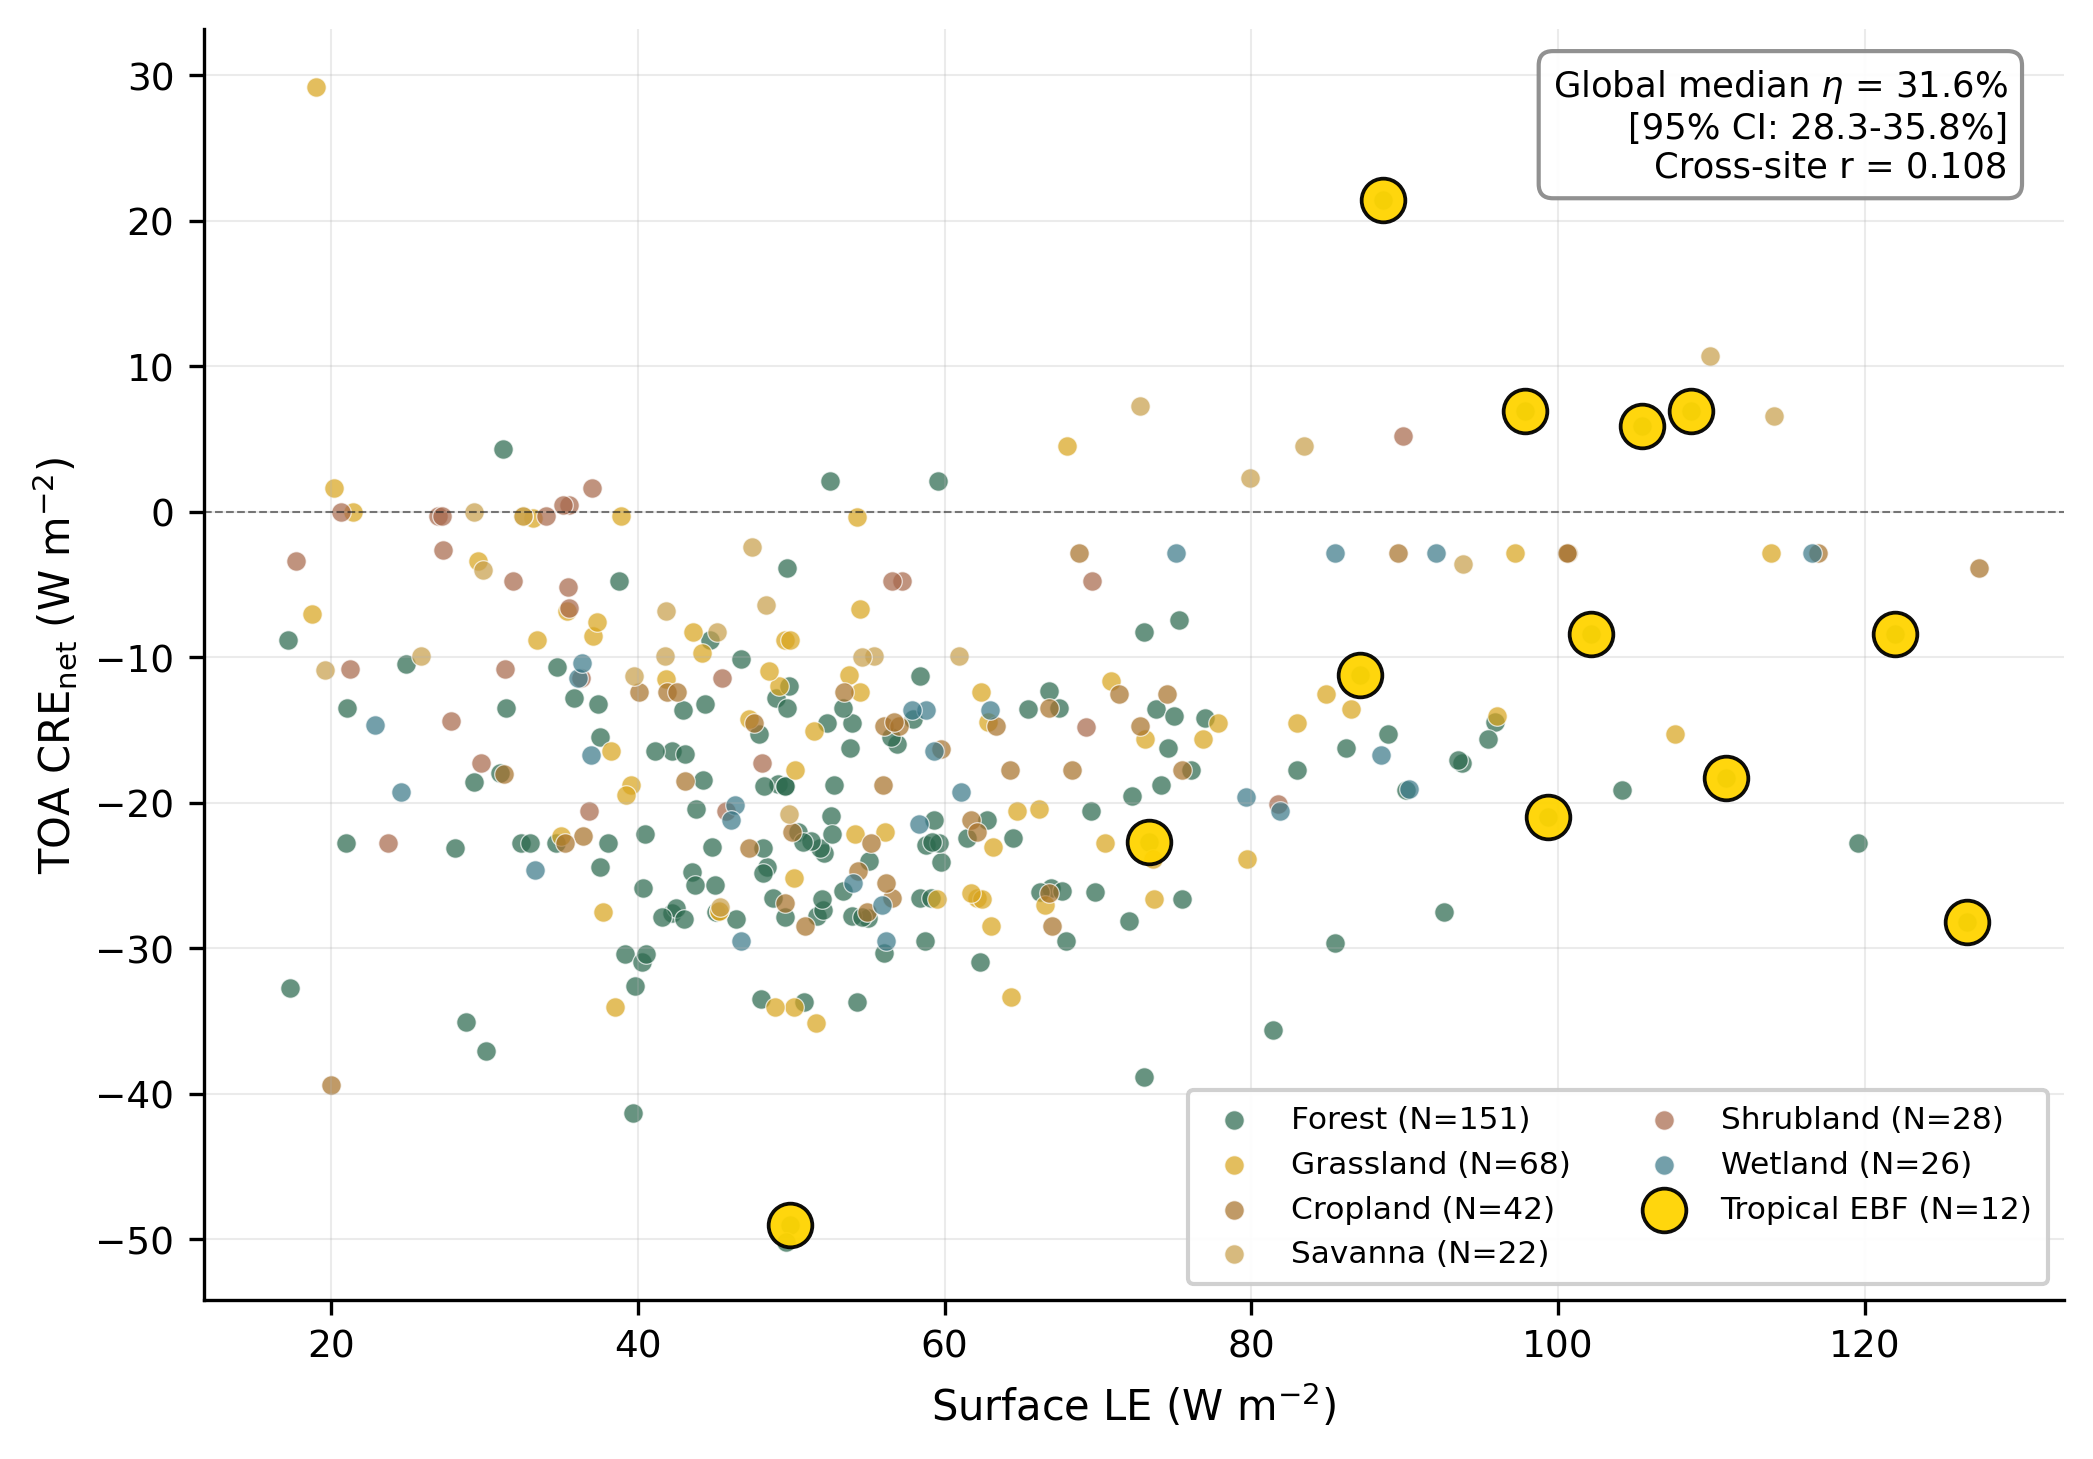
\includegraphics[width=6.5in,height=5.58209in]{./figures/fig2_le_vs_cre_net_notitled.png}

\emph{Figure 2. Surface LE versus TOA CRE\_net across 341 FLUXNET-CERES
co-located sites. Points coloured by biome. Tropical evergreen broadleaf
forest sites shown with yellow markers. The transfer fraction η =
\textbar CRE\_net\textbar{} / LE is the slope of the relationship within
each biome. The global median η = 31.6\% {[}95\% CI: 28.3 to 35.8\%{]}.
Note: the cross-site correlation between LE and CRE\_net is near-zero (r
= 0.029); the transfer fraction is the within-biome ratio, not the OLS
slope of the scatter.}

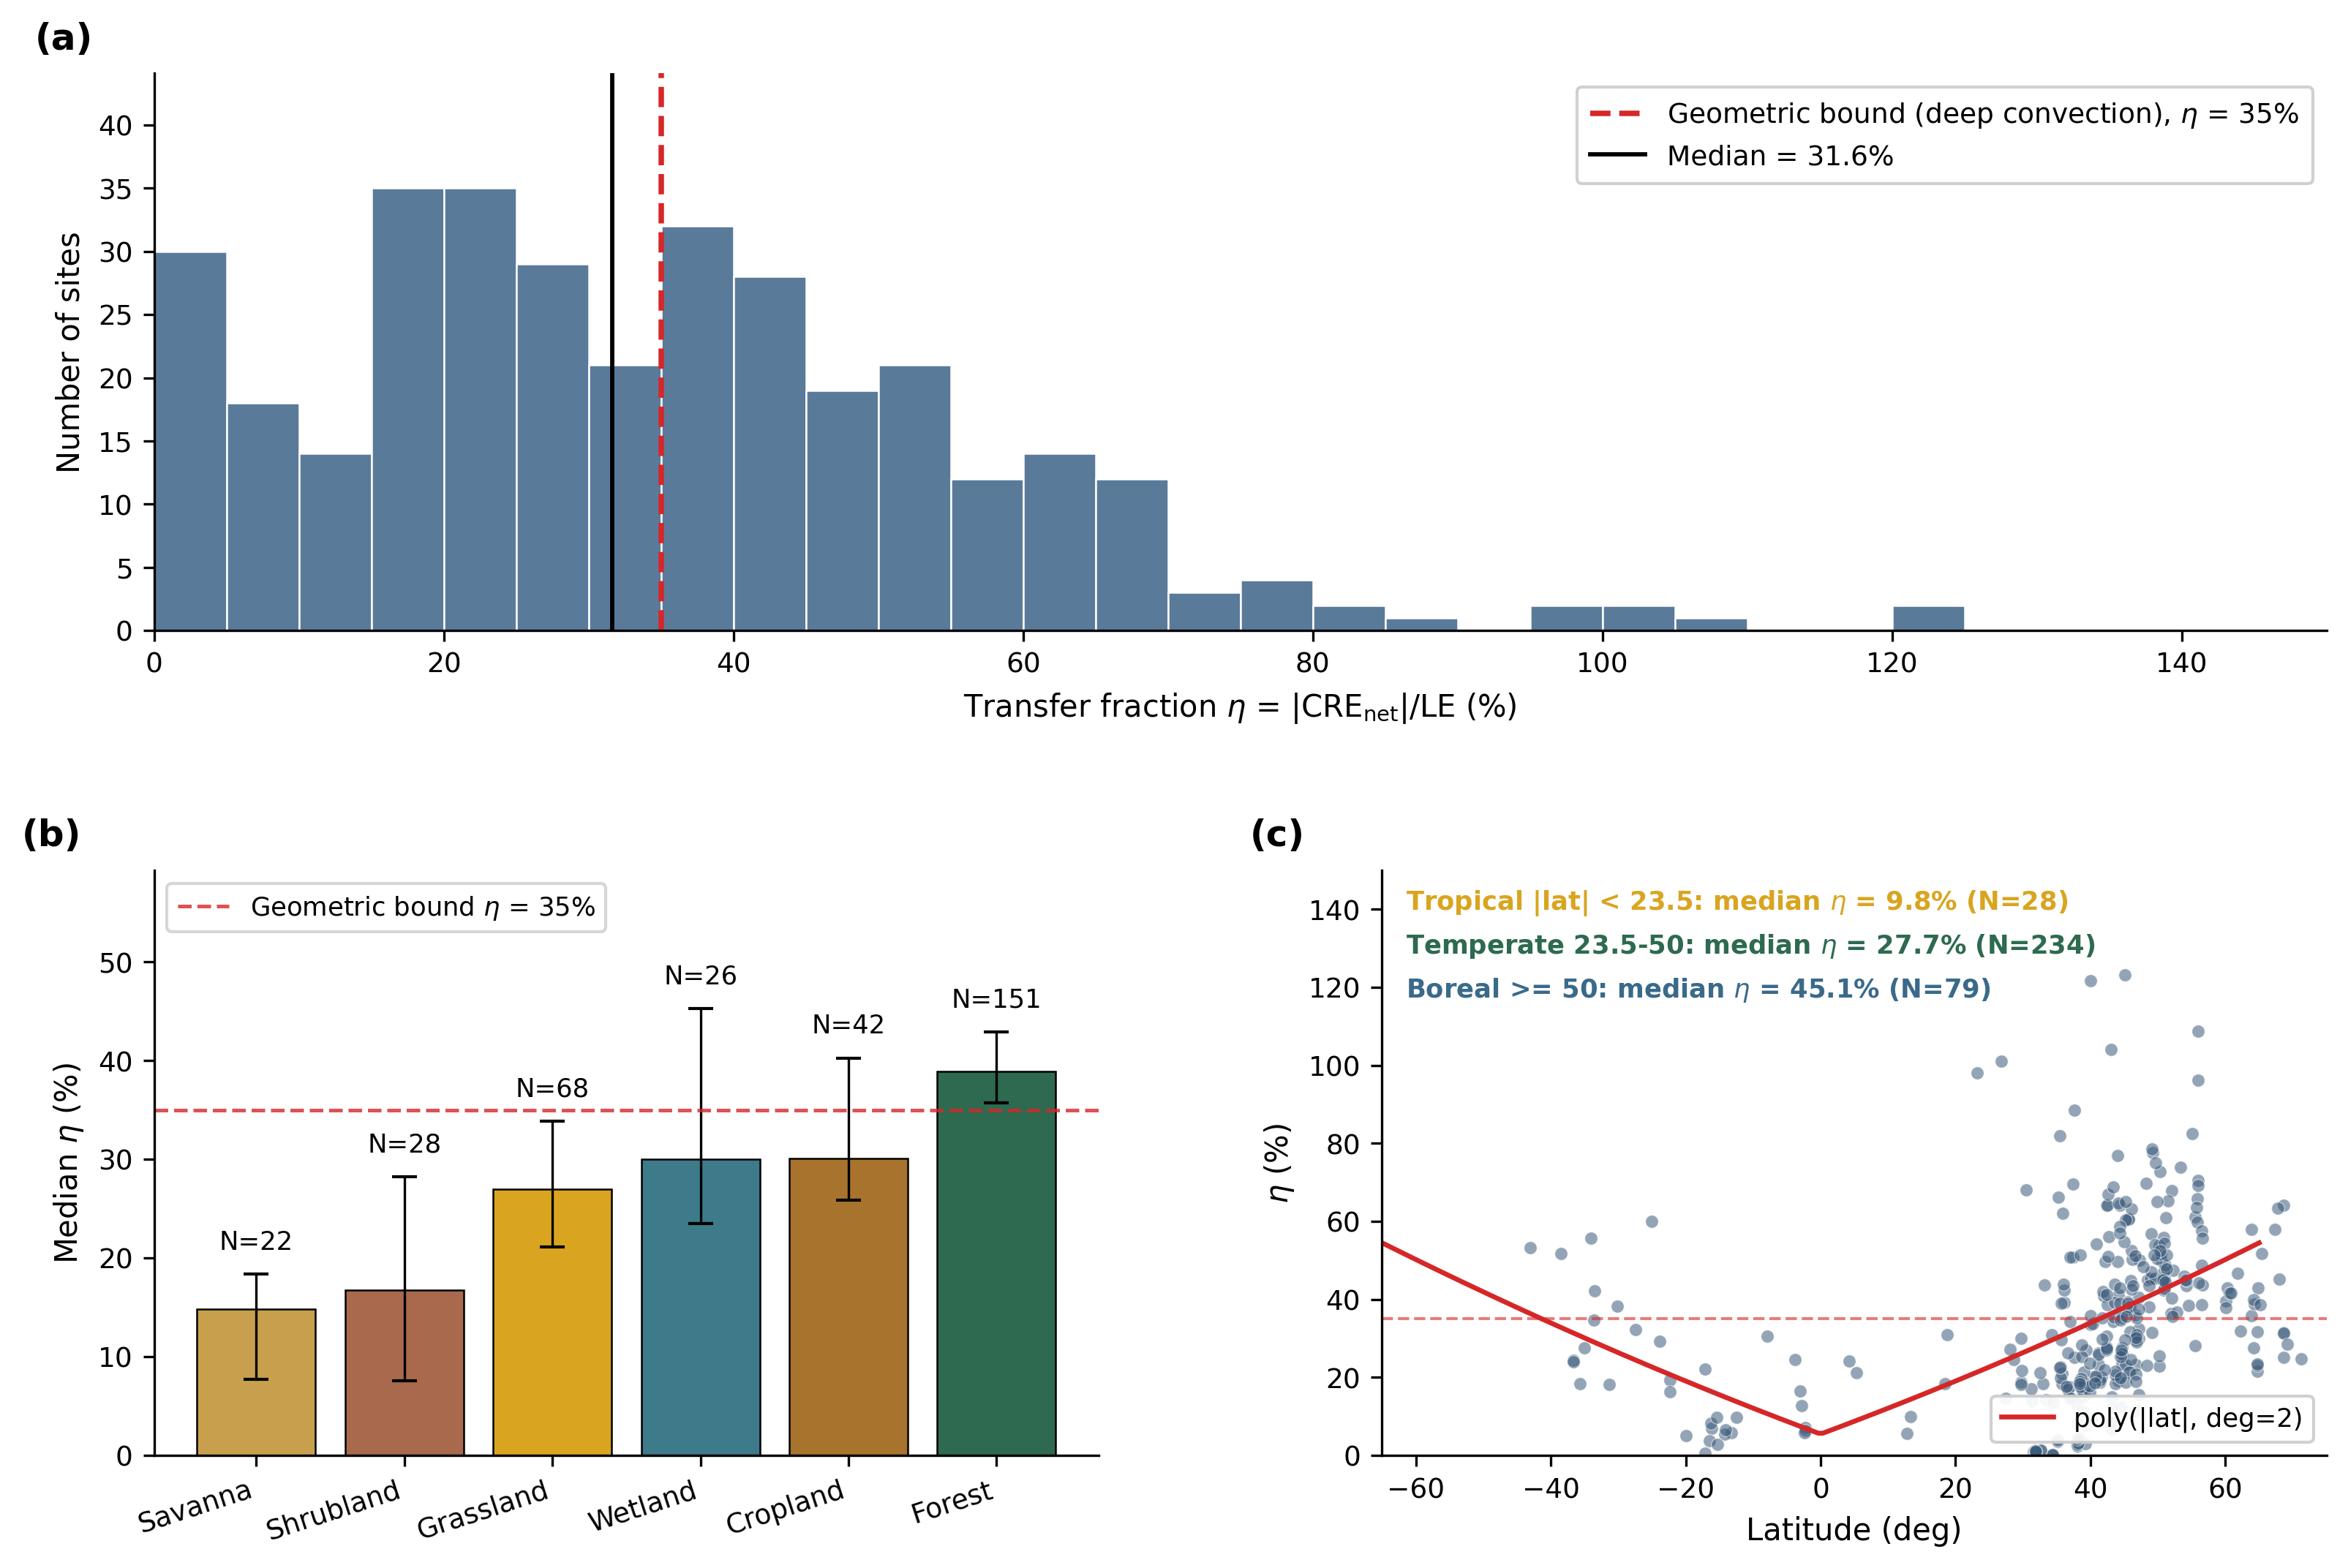
\includegraphics[width=6.5in,height=5.53102in]{./figures/fig3_global_consistency_notitled.png}

\emph{Figure 3. Global consistency of the transfer fraction. (a)
Histogram of η across all 341 sites. (b) Median η
by biome with bootstrap 95\% CI. (c) η versus latitude, with tropical
(\textbar lat\textbar{} \textless{} 23.5°), temperate, and boreal
medians annotated. Dashed line indicates the 35\% basin-scale
reference bound derived for tropical deep-convective regimes
(Section 6.10).}

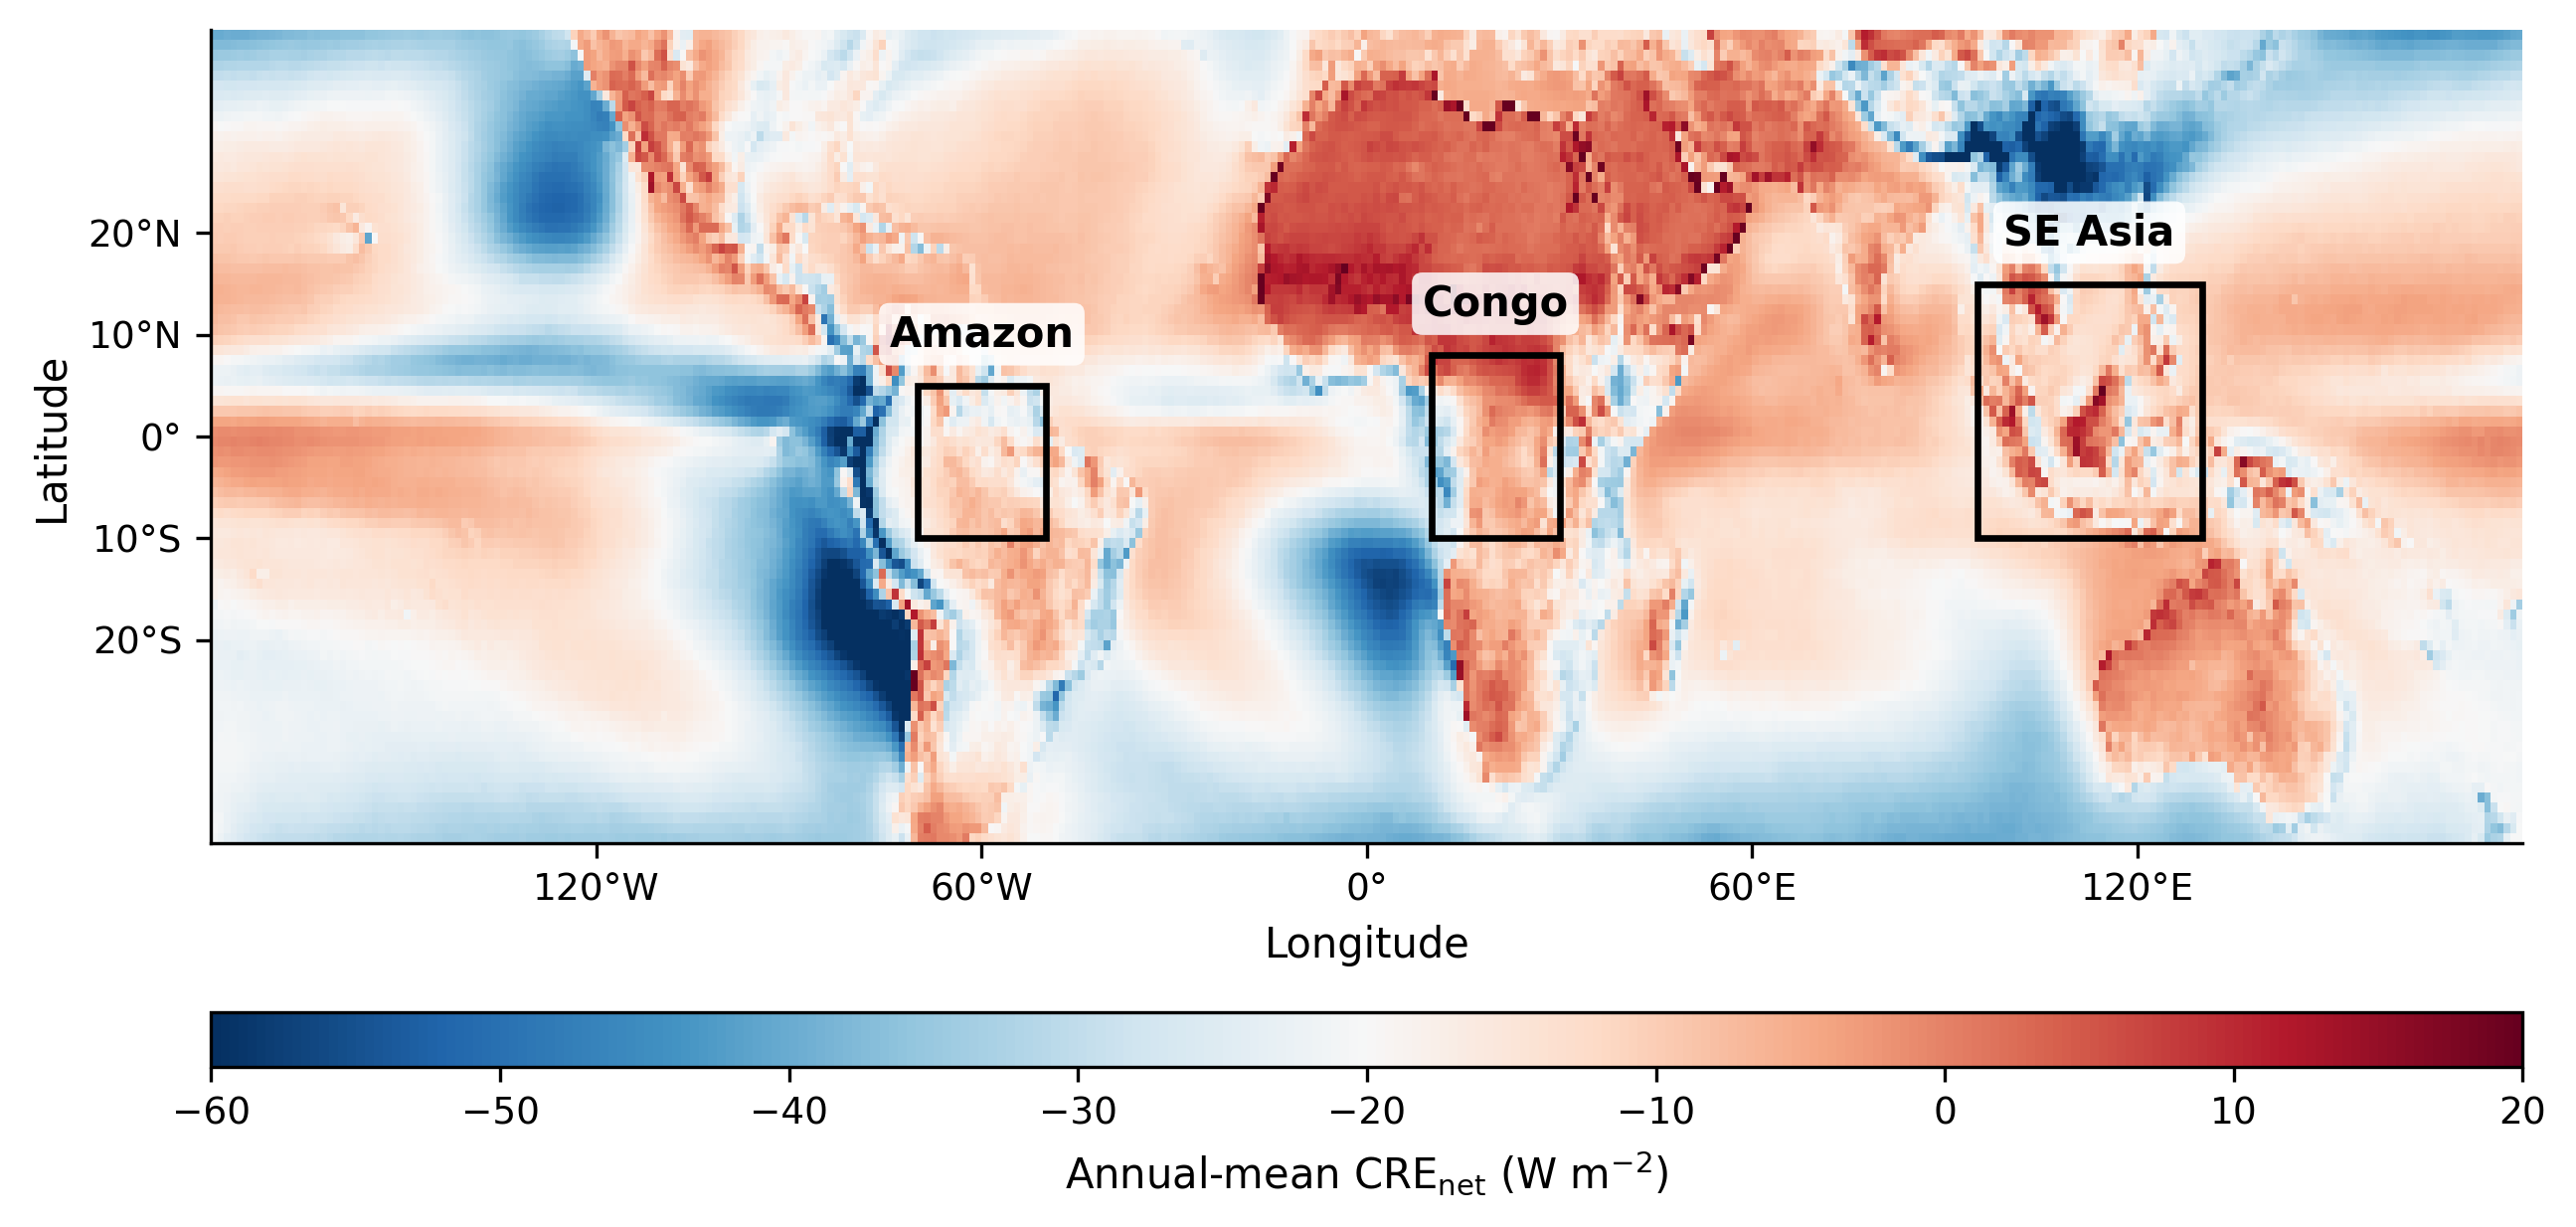
\includegraphics[width=6.5in,height=2.52948in]{./figures/fig4_study_regions_notitled.png}

\emph{Figure 4. Study regions overlaid on annual mean CRE\_net from
CERES EBAF Ed4.2 (2003--2023). Blue shading indicates net TOA cooling;
red indicates net warming. Basin extraction polygons for the Amazon,
Congo, and SE Asia are outlined.}

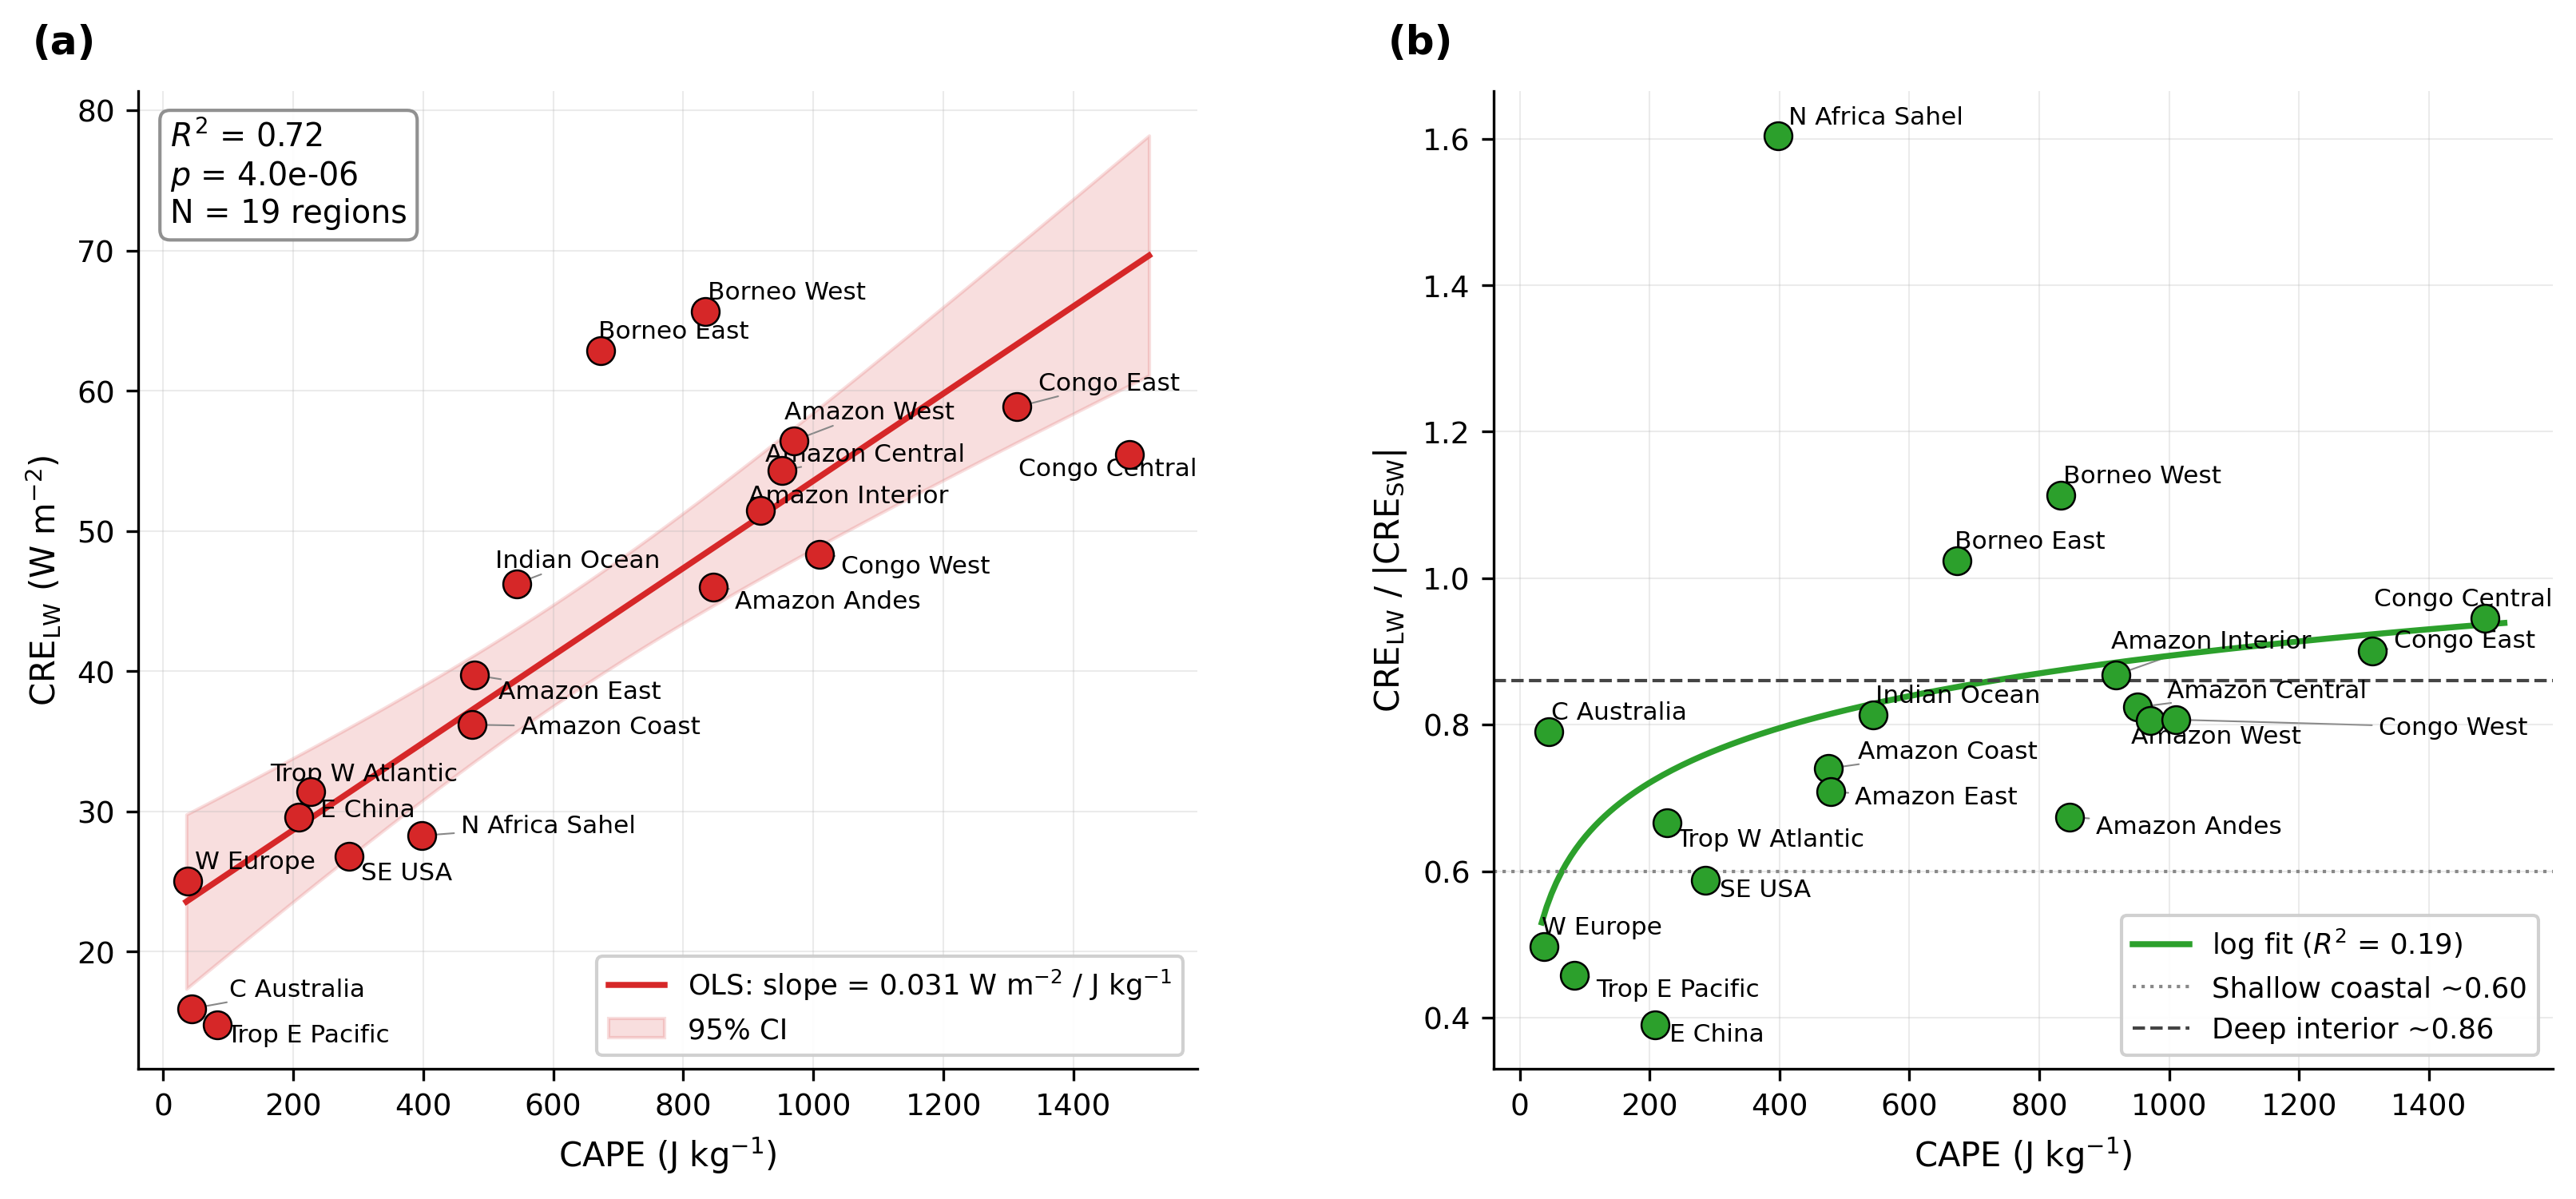
\includegraphics[width=6.5in,height=2.98522in]{./figures/fig5_cape_cre_lw_notitled.png}

\emph{Figure 5. CRE\_LW attenuation mechanism. (a) CRE\_LW versus CAPE
across 19 regions (R² = 0.74, p = 2.4 × 10⁻⁶). 95\% confidence band
shown. (b) CRE\_LW/\textbar CRE\_SW\textbar{} ratio converges toward 1.0
with convective depth.}

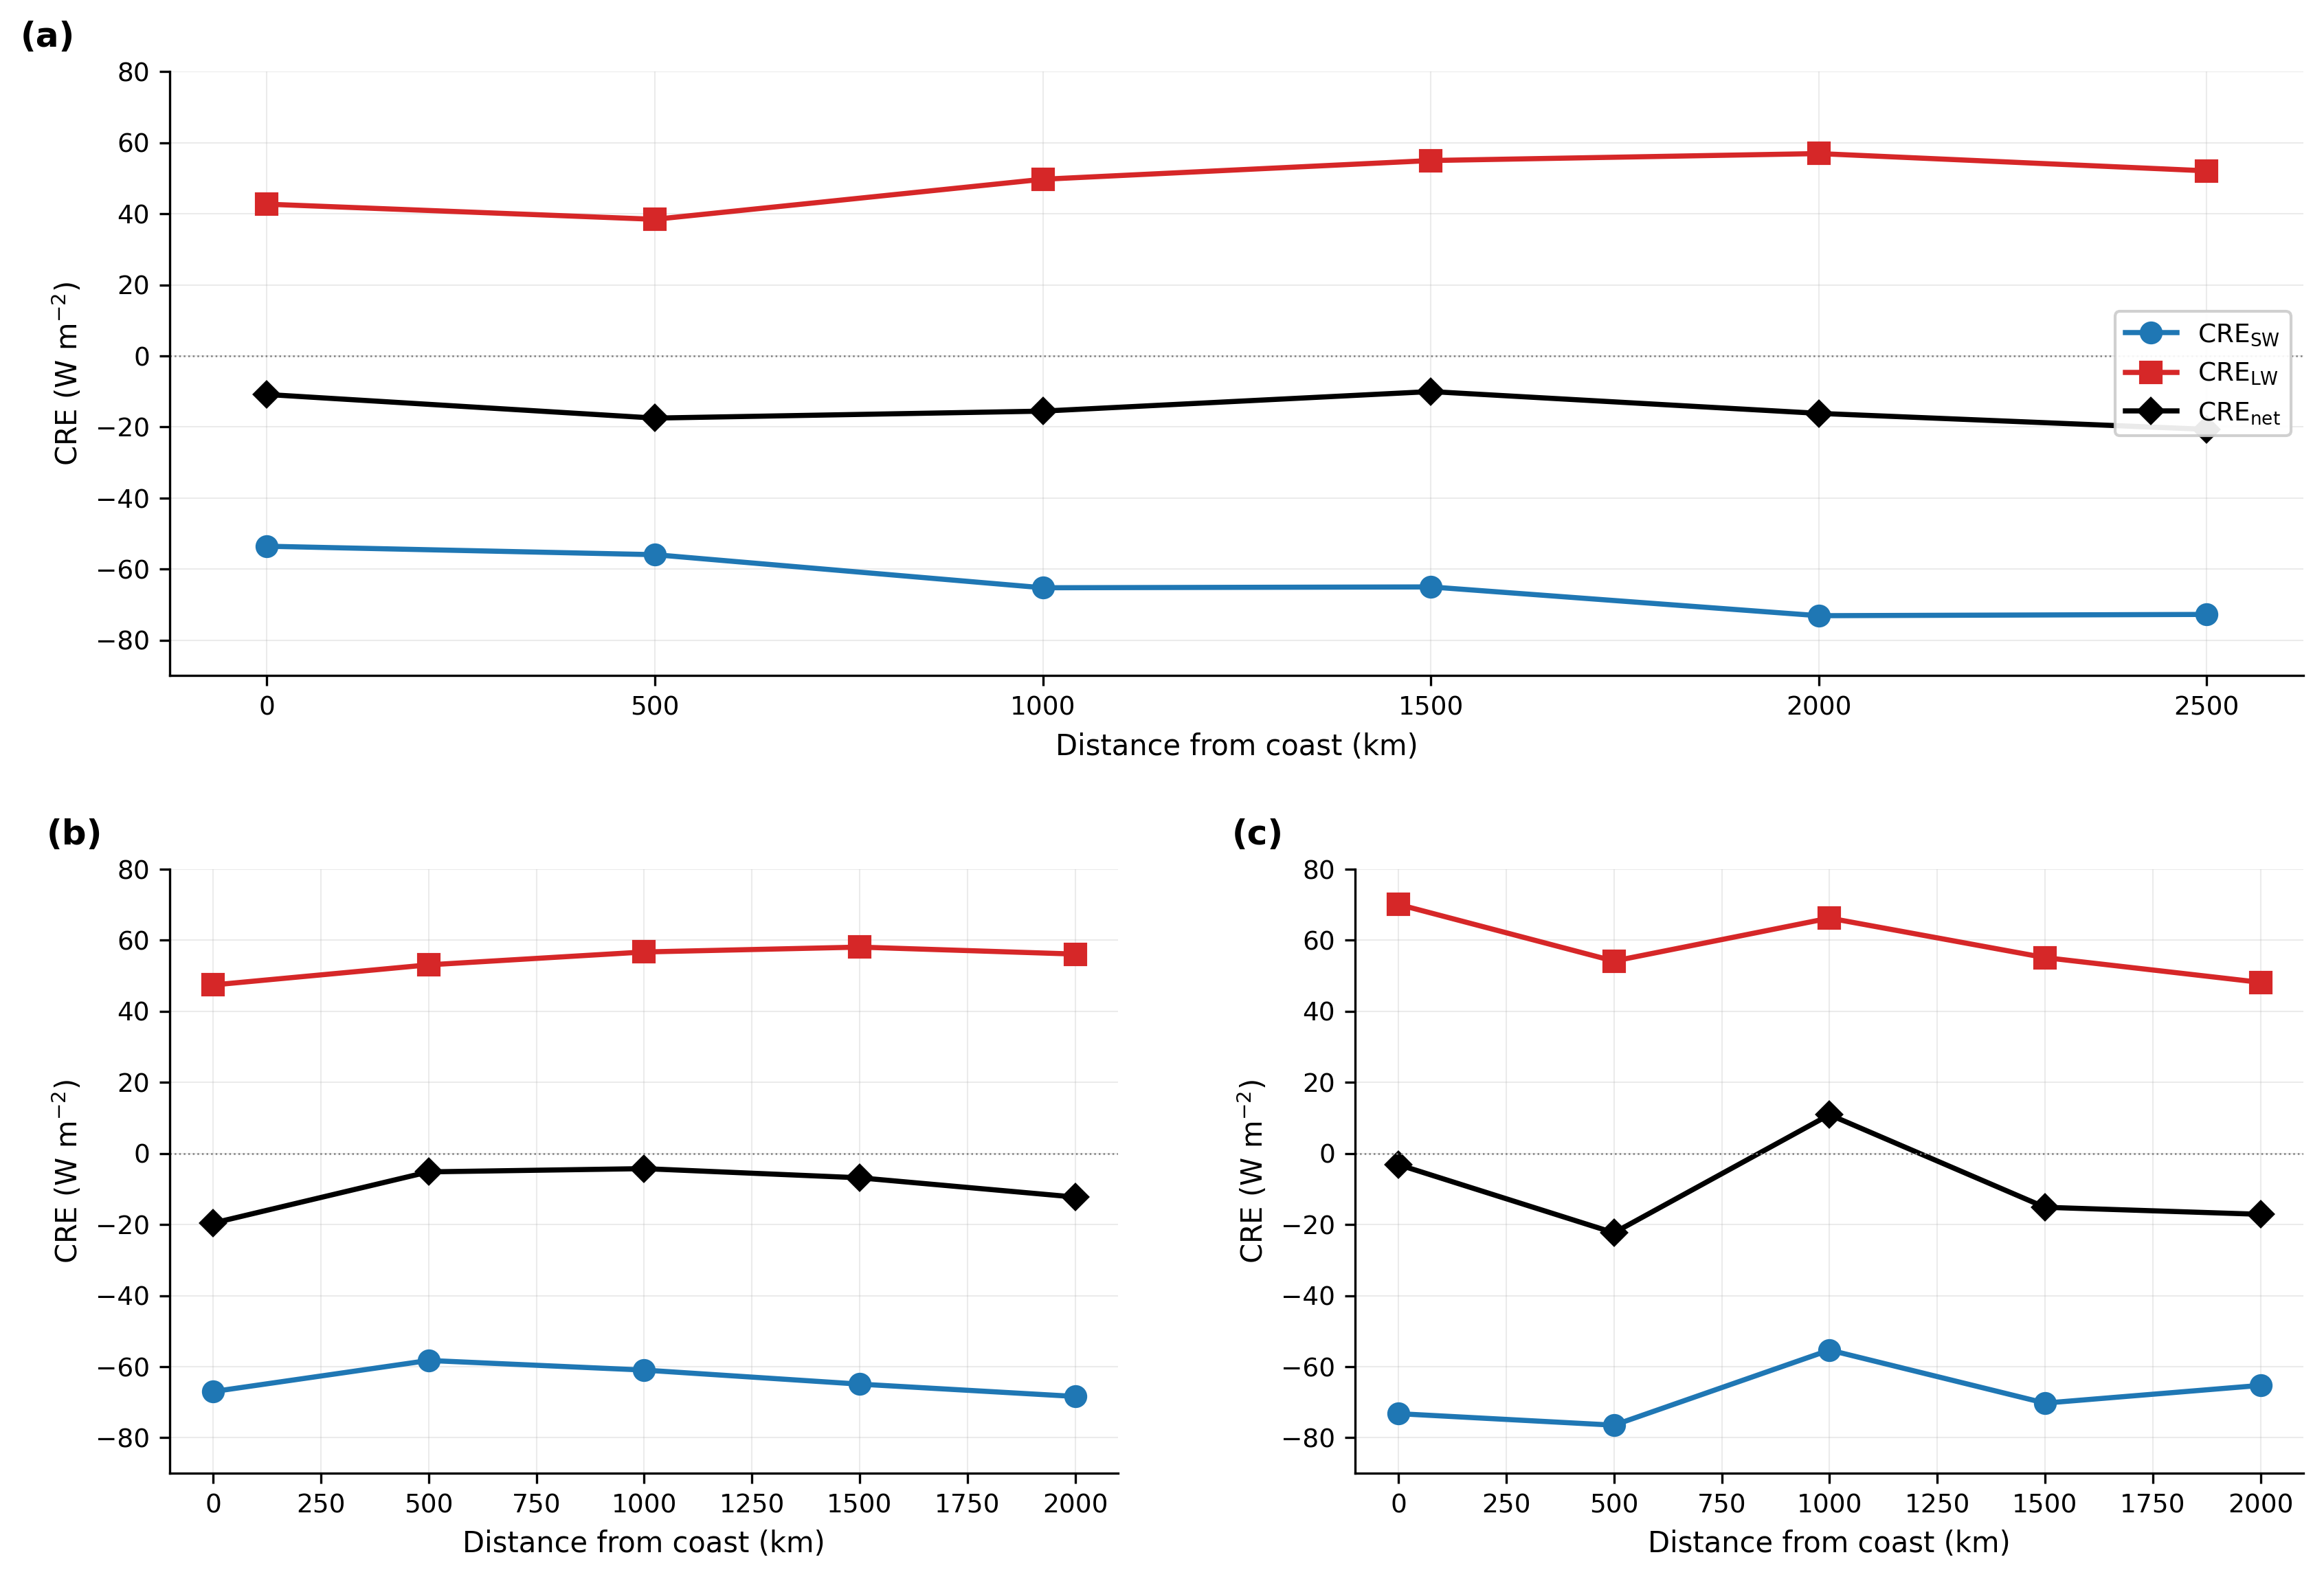
\includegraphics[width=6.5in,height=2.31138in]{./figures/fig6_cross_basin_transects_notitled.png}

\emph{Figure 6. Cross-basin transects for the Amazon, Congo, and SE
Asia. Each panel shows CRE\_SW, CRE\_LW, and CRE\_net (W~m⁻²) as a
function of distance from the coast. CRE\_SW and CRE\_LW intensify
together (lockstep), while CRE\_net remains approximately flat. This
pattern is reproduced in all three basins.}

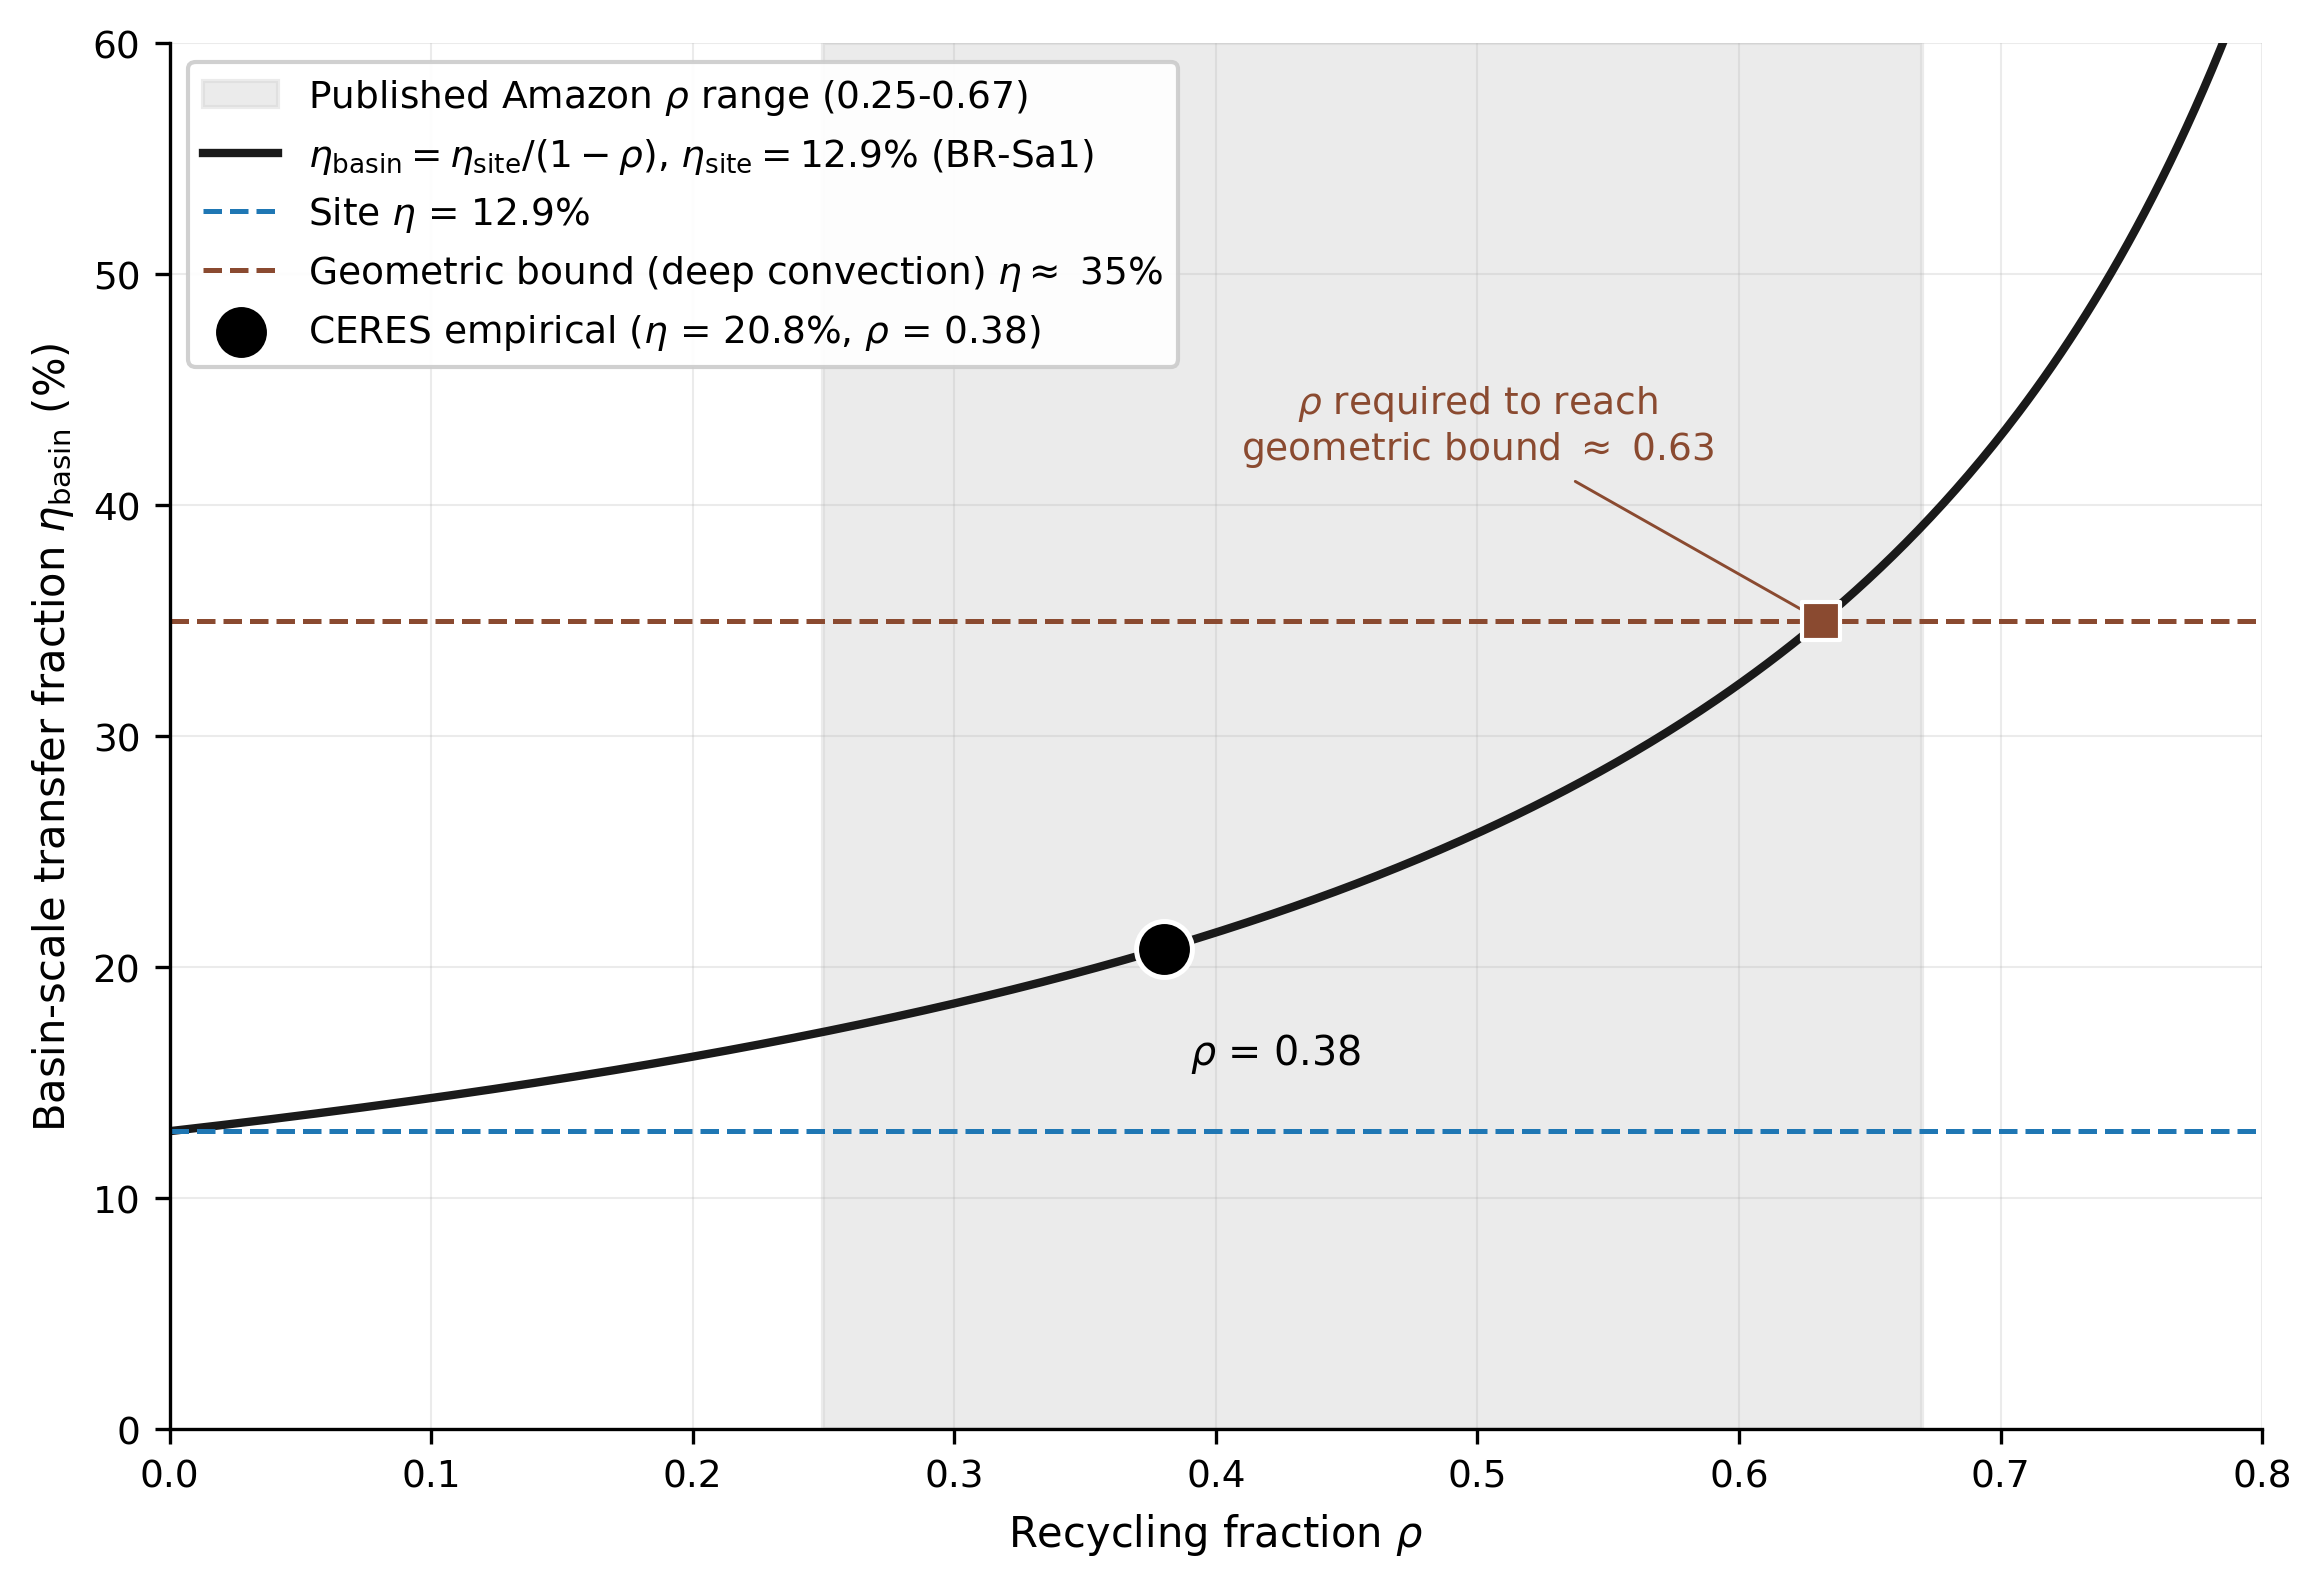
\includegraphics[width=6.5in,height=4.8454in]{./figures/fig7_recycling_amplification_notitled.png}

\emph{Figure 7. Recycling amplification model and CERES validation.
Theoretical η\_basin as a function of recycling fraction f. Published
estimates marked. Basin empirical value (20.8\%) consistent with f =
38\%. The 35 percent geometric bound (red dashed) requires ρ ≈ 0.58, within the published Amazon recycling range of 0.25 to 0.67.}

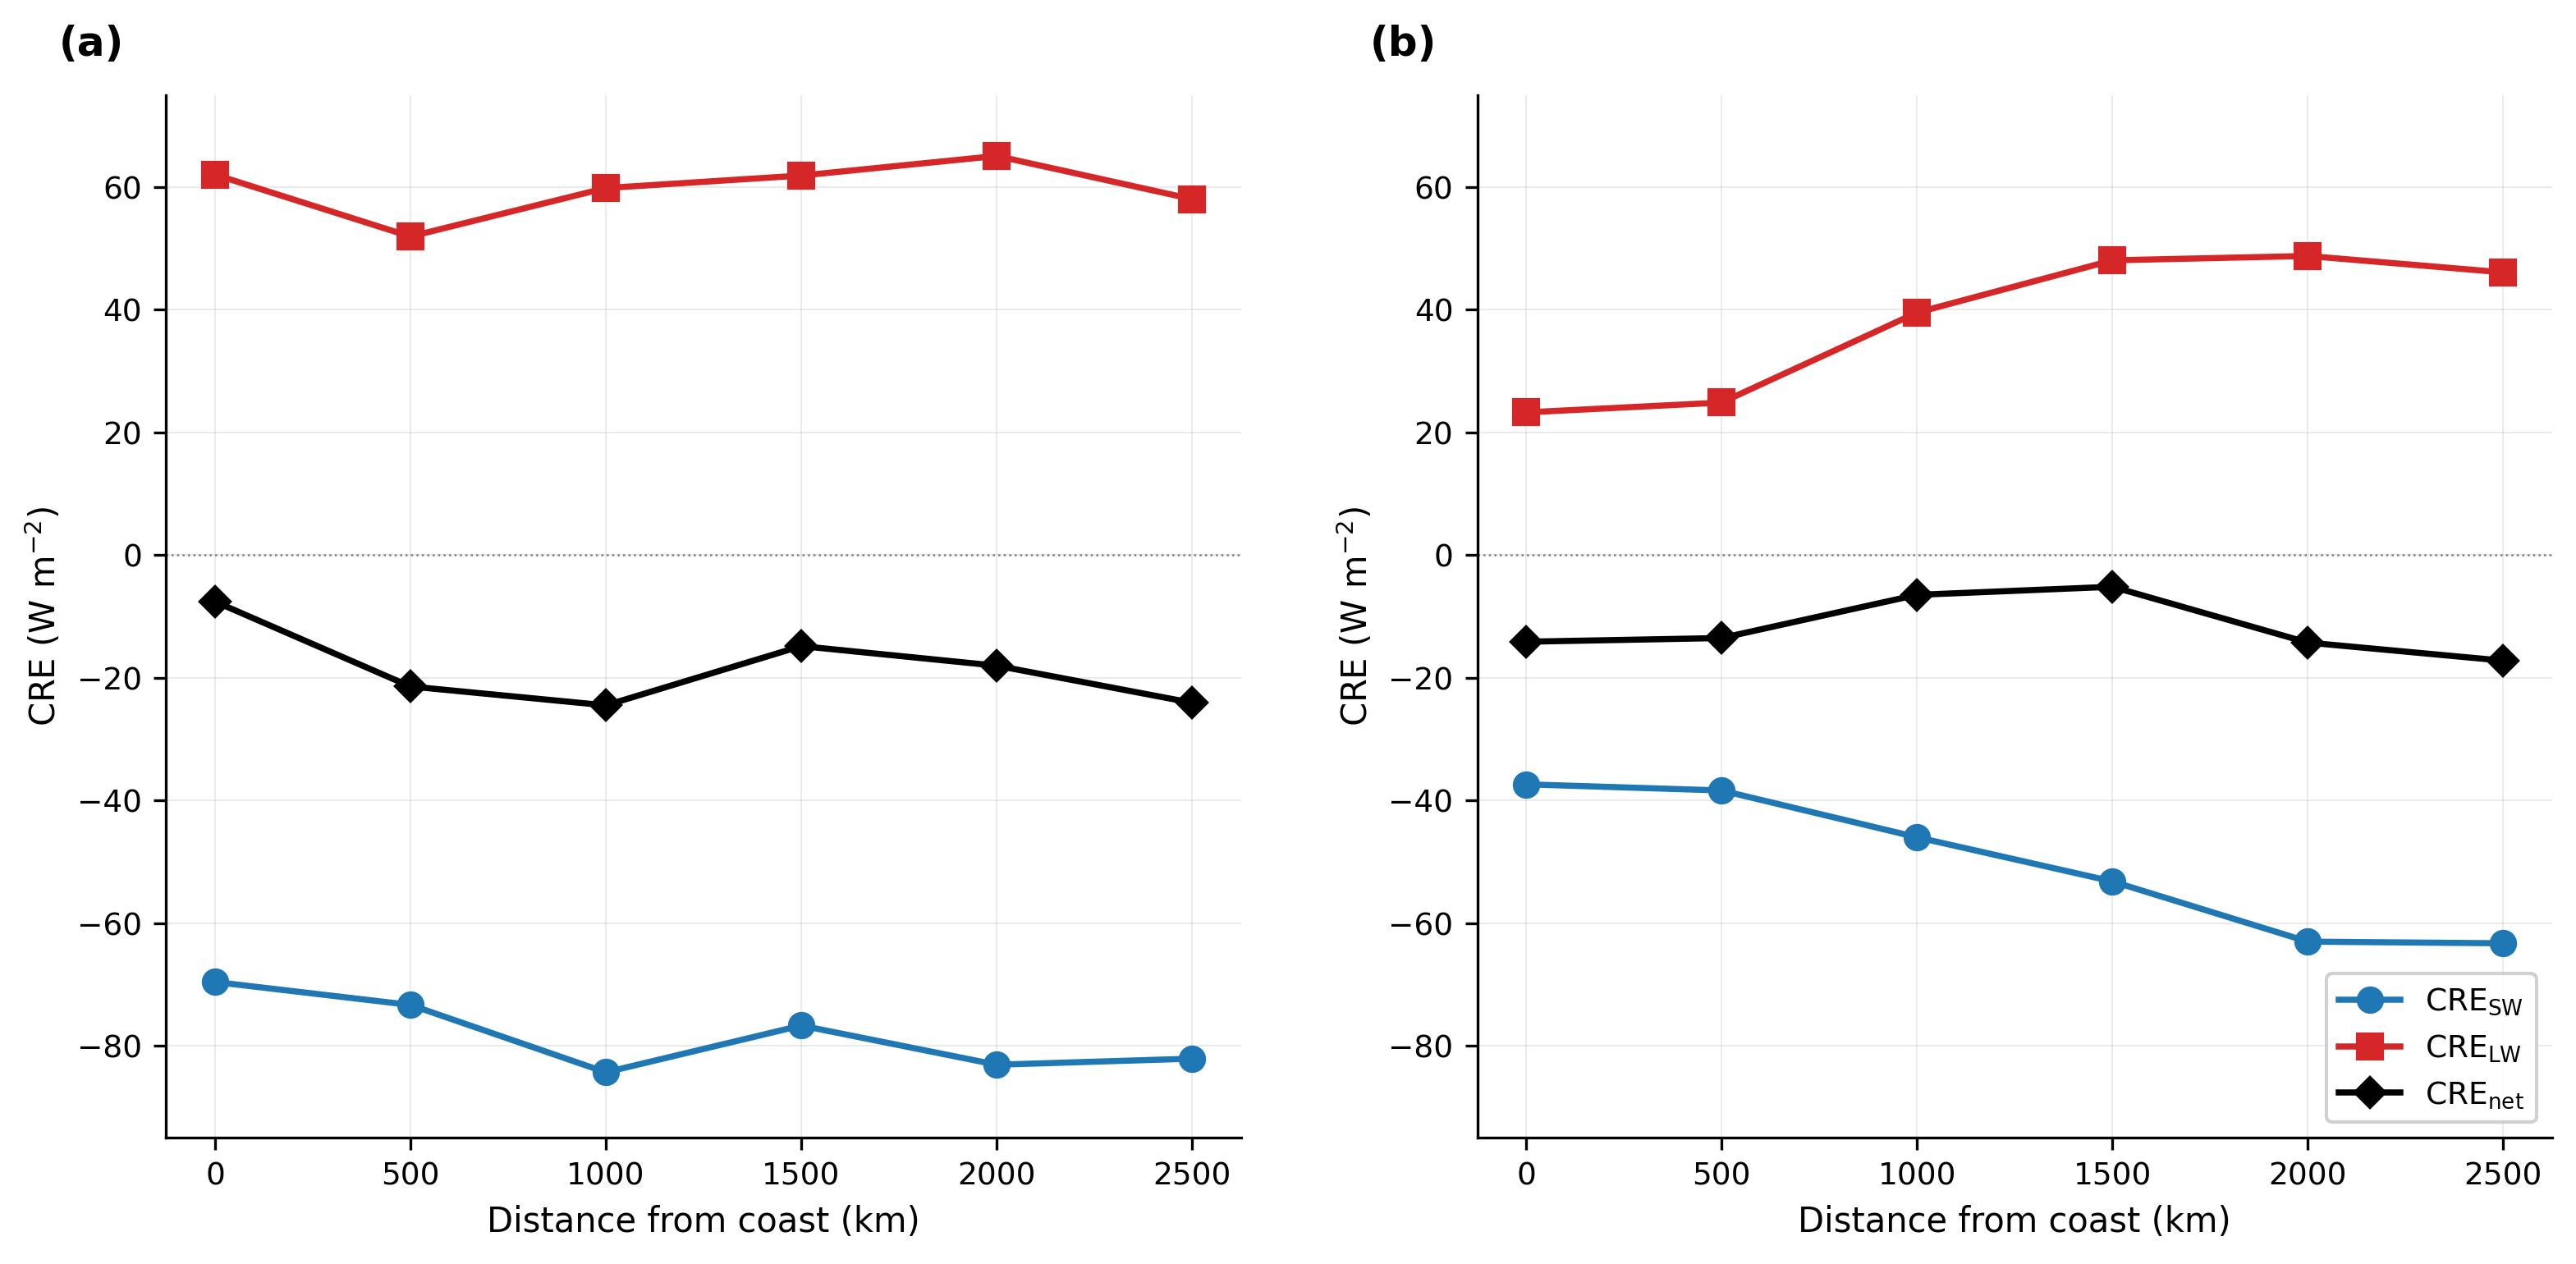
\includegraphics[width=6.5in,height=2.64468in]{./figures/fig8_seasonal_transect_notitled.png}

\emph{Figure 8. Seasonal Amazon transect. (a) Wet season (DJF-MAM):
uniformly high CRE. (b) Dry season (JJA-SON): coast loses cloud cover
(54\%), interior retains it (78\%). The steeper dry-season gradient is
the biotic pump signature.}

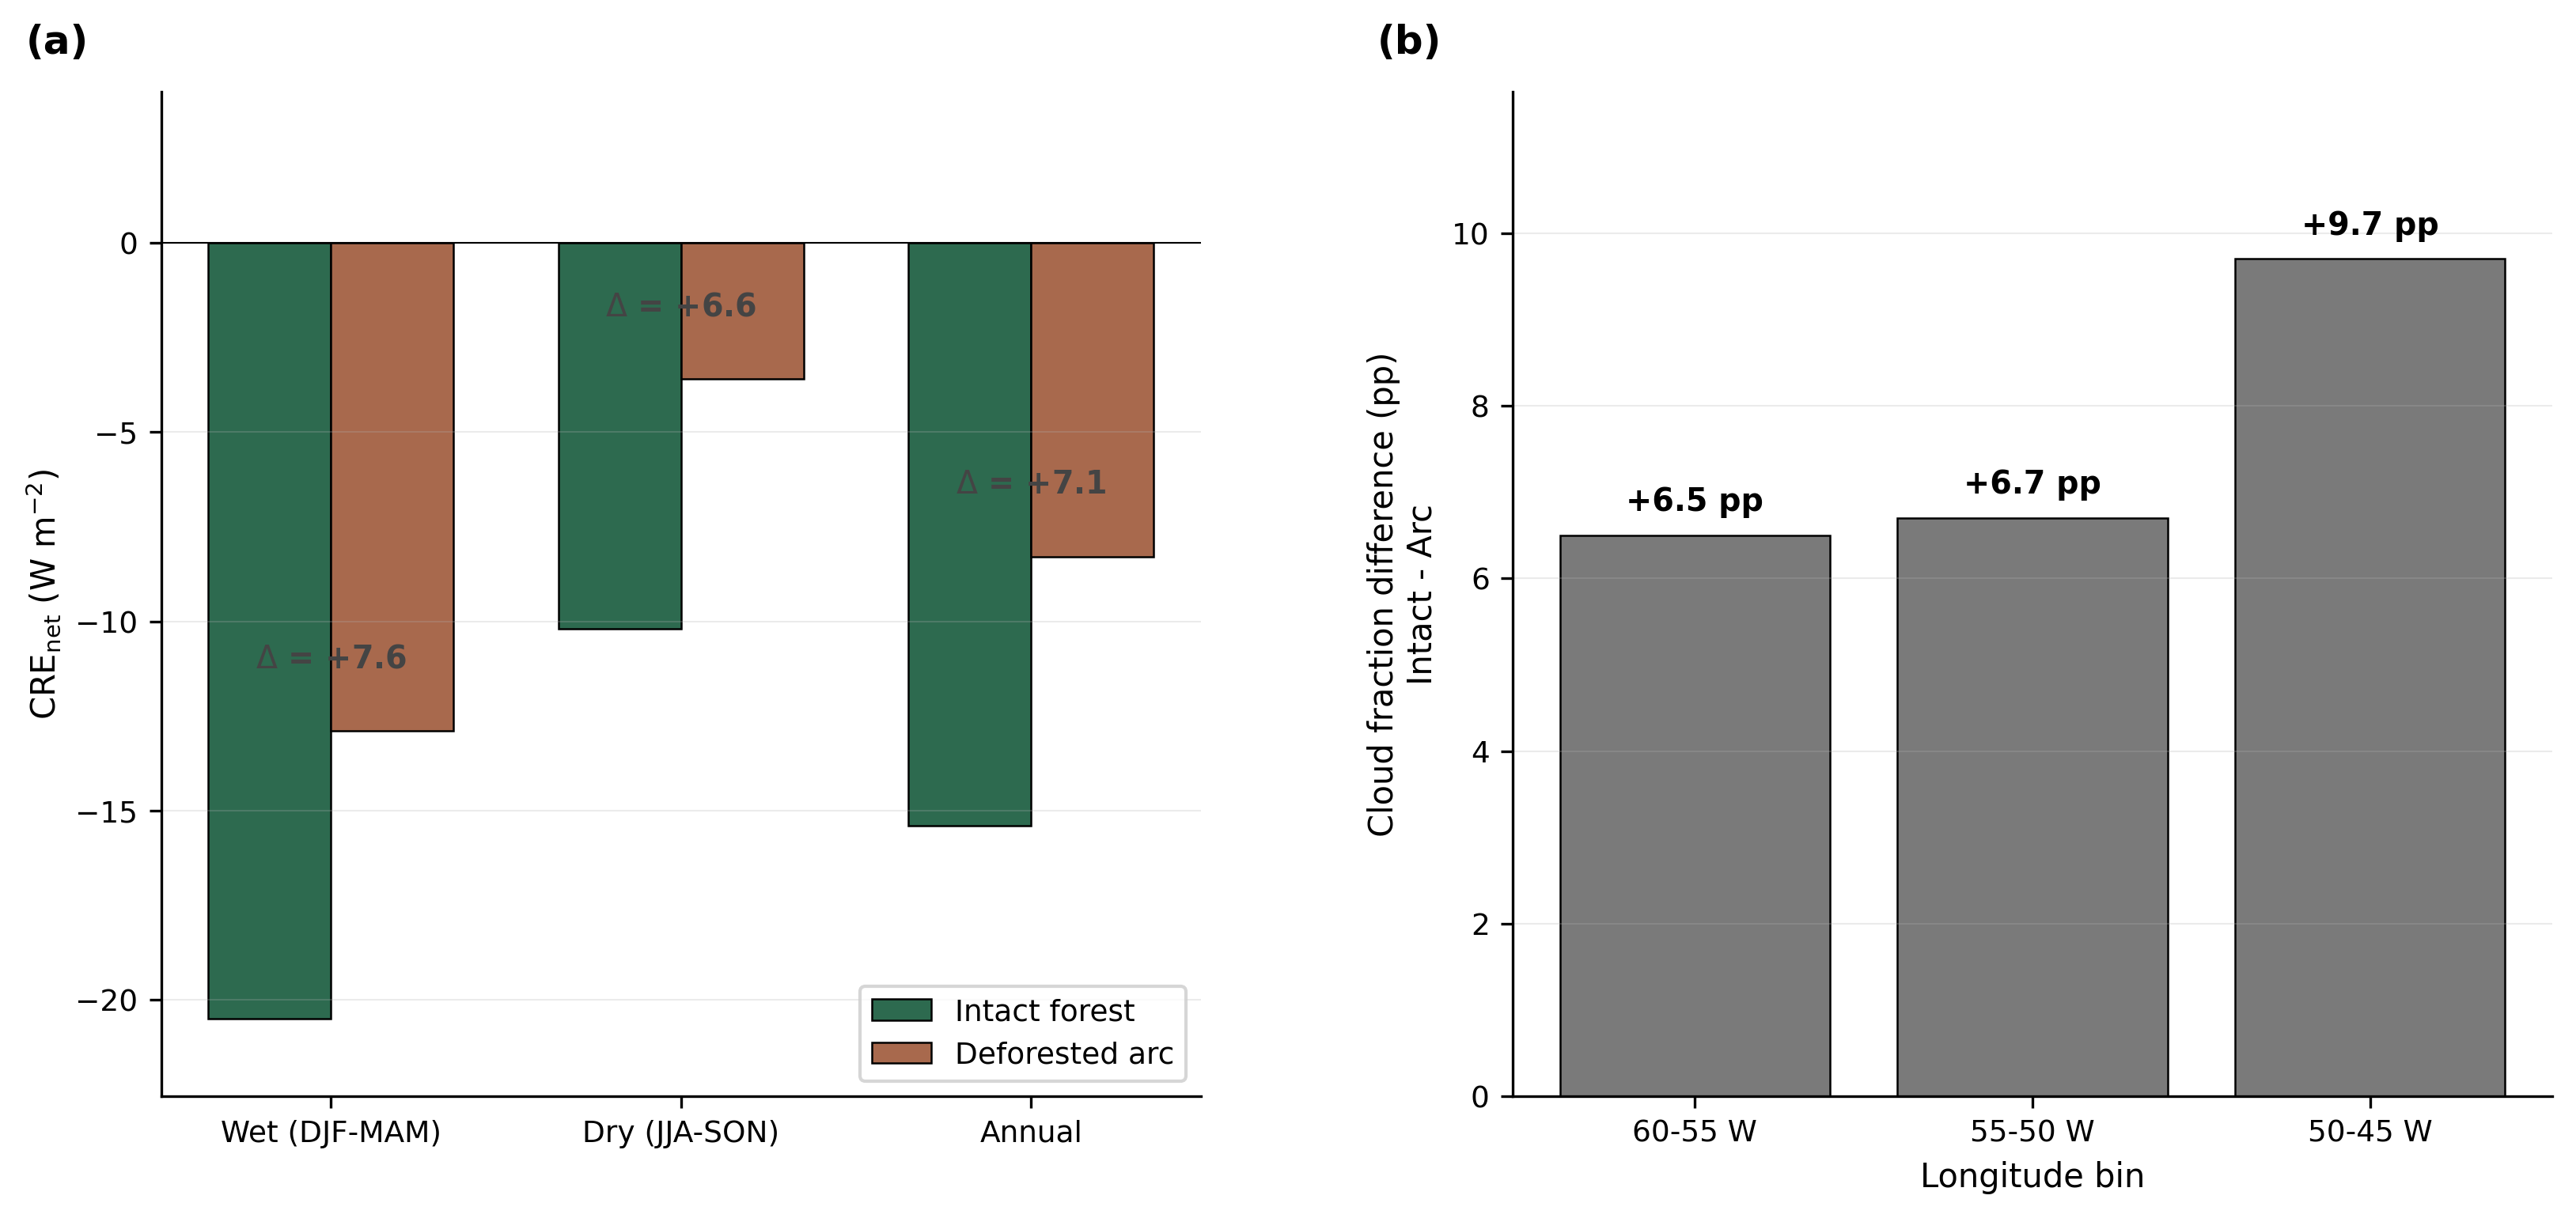
\includegraphics[width=6.5in,height=2.85091in]{./figures/fig9_deforestation_counterfactual_notitled.png}

\emph{Figure 9. Deforestation counterfactual. (a) CRE\_net (W~m⁻²) for
intact Amazon forest versus deforested arc. (b) Cloud fraction
difference: 6.5 to 9.7 percentage points.}

\textbf{7. Conclusions}

This study provides a dedicated, scale-stratified observational
constraint on the fraction of surface latent heat flux reaching the
top of atmosphere as net radiative cooling, extending the preliminary
site-level regression estimate of Shahid (2026b) to basin scale across
341 sites globally and adding a mechanistic decomposition and
geometric bound. Six conclusions follow from the analysis.

1. \emph{Site-level constraint.} The median transfer fraction for
tropical evergreen broadleaf forest is $\eta = 14.7\%$ (range 5.6 to
31.0\% across 12 sites spanning 5 continents); the Amazon flagship
site BR-Sa1 yields 12.9\%. Across the full 341-site FLUXNET cross-
biome sample, the global median is $\eta = 31.6\%$, confirming that
low single-digit to low double-digit values are characteristic of
moist tropical systems rather than artifacts of site selection.

2. \emph{Basin-level constraint.} The basin-integrated transfer
fraction for the Amazon is 20.8\% (CRE\_net = $-19.8$ W~m$^{-2}$, LE
= 95.1 W~m$^{-2}$), with a moisture recycling amplification of
$1.62\times$ relative to the single-site value. Cross-basin
replication yields Congo $1.63\times$ and SE Asia $1.57\times$. These
are, to our knowledge, the first basin-integrated observational
transfer fractions reported for the world's three major tropical
forest basins.

3. \emph{Geometric bound mechanism.} CRE\_LW scales with CAPE at
$R^2 = 0.74$ (slope 0.032 W~m$^{-2}$ per J~kg$^{-1}$), and CRE\_SW
and CRE\_LW intensify in lockstep along coast-to-interior transects
in all three basins with CRE\_net remaining approximately flat. This
CRE\_SW/CRE\_LW lockstep is a universal feature of deep convective
regimes and imposes a geometric upper bound on $\eta$ that cannot be
circumvented by moisture recycling or large-scale transport.

4. \emph{Biotic pump observational fingerprint.} Interior Amazon
forest maintains cloud cover at CRE\_SW = $-60$ W~m$^{-2}$ in the
dry season while the coast declines to $-37$ W~m$^{-2}$. This
east-west seasonal gradient is the observational fingerprint of the
biotic pump mechanism, consistent with Makarieva and Gorshkov (2007),
Ellison et al. (2025), and the vertical-coherence framework of Shahid
(2026c).

5. \emph{Deforestation signal.} Deforestation in the Amazon arc
yields a CRE\_net penalty of 2.6 to 11.5 W~m$^{-2}$ and a cloud
fraction reduction of 6.5 to 9.7 percentage points relative to
intact forest, demonstrating that forest loss produces a measurable
and quantifiable impact on the TOA radiation budget.

6. \emph{Scale-dependent applications.} The transfer fraction
operates simultaneously as a cloud feedback diagnostic and as
the TOA counterpart to the surface biophysical forcing coefficient
$\alpha(\beta)$. The 1.62$\times$ recycling amplification from site to
basin scale is a physical property of the η-ρ system, independent of
any particular valuation framework. Translating this scale-dependent
physical envelope into per-hectare radiative value, with the auxiliary
assumptions on social cost of carbon and counterfactual land cover,
is the subject of Paper 8 (cascade valuation).

The present paper (Paper~6) closes the LE-specific vertical transfer arm of a broader
programme on surface-to-atmosphere energy coupling. Paper~1
established the surface forcing coefficient $\alpha(\beta)$ (Shahid
2026a); Paper~2 tested whether $\alpha(\beta)$ propagates to TOA
cloud radiative effects across 314 FLUXNET sites (Shahid 2026b);
Paper~3 characterised the horizontal moisture corridors that sustain
inland rainfall in the Amazon and Congo basins (Shahid 2026c). The
present paper extends the site-level propagation test of Paper~2 to
basin scale and adds the cloud-mediated mechanistic decomposition. Four companion studies are in
preparation and round out the programme. Paper~4 examines the
Andes Low-Level Jet and ENSO modulation of basin-scale transfer.
Paper~5 quantifies edge effects in fragmented tropical landscapes.
Paper~8 develops cascade valuation across nested spatial scales.
Paper~9 targets event-scale radiative responses to individual
convective systems. Together these lines of work extend the
framework from steady-state climatology toward the dynamical and
economic regimes in which forests actually operate.

\textbf{Acknowledgements}

This study uses data products from several open-access observational
networks and reanalysis programmes.

\textit{Surface flux observations.} The FLUXNET2015 and ONEFlux datasets
are used with acknowledgement to the FLUXNET community, its regional
flux networks (AmeriFlux, AsiaFlux, CarboEuropeIP, ChinaFlux, LBA,
OzFlux, and others), and the individual site principal investigators who
collect, quality-control, and openly distribute eddy-covariance
measurements. The LBA project provided the Amazon tower measurements
(BR-Sa1 and BR-Sa3 at Tapajós). Data processing and standardisation
were supported by the FLUXNET2015 and ONEFlux collaborations, the
European Fluxes Database Cluster, and the Integrated Carbon Observation
System (ICOS).

\textit{TOA radiation.} CERES EBAF Edition~4.2 TOA radiation data were
obtained from the NASA Langley Research Center Atmospheric Science Data
Center (https://ceres.larc.nasa.gov/). The CERES programme is
acknowledged for sustained provision of calibration-stable multi-decadal
radiation records.

\textit{Atmospheric reanalysis.} ERA5 reanalysis data were obtained from
the Copernicus Climate Change Service Climate Data Store
(https://cds.climate.copernicus.eu/) and were produced by the European
Centre for Medium-Range Weather Forecasts (ECMWF) under the Copernicus
programme of the European Union. Hersbach et al.\ (2020) describe the
ERA5 production system.

\textit{Land cover.} MODIS MCD12C1 land cover product was obtained from
NASA Land Processes Distributed Active Archive Center (LP DAAC,
https://lpdaac.usgs.gov/).

\textit{Upstream programme data products.} The joined FLUXNET-CERES
site summary used in this study was produced by the Paper~1 data
pipeline (Shahid, 2026a); details of the joining procedure and
per-site processing are described in that paper's methods and code
archive.

\textbf{Data and Code Availability}

Data products used in this study are openly available from the sources
listed above. The analysis pipeline, figure-build scripts, and the 10
result tables cited in the paper are archived at
\url{https://github.com/R3GENESI5/shahid-2026-transfer-fraction}. The
repository is private during peer review and will be made public on
acceptance; reviewer access is available on request. A Zenodo archive
of the repository at the version of record will be deposited on
acceptance and the DOI added to this section at proof stage. No new
primary observations were collected for this study; all quantitative
results are reproducible from the archived code and the listed data
sources.

\textbf{Author Contributions}

A.B.S. designed the study, assembled the joined FLUXNET-CERES dataset,
performed the analysis, generated the figures, and wrote the
manuscript.

\textbf{Competing Interests}

The author declares no competing interests.

\textbf{AI Usage Disclosure}

Large-language-model assistants (Anthropic Claude, version Opus) were
used during manuscript preparation for literature-review drafting,
reference-list formatting and Crossref verification, figure
build-script review and stylistic editing, cross-section consistency
checks, and internal adversarial review of numerical claims. All
substantive scientific content (study design, data selection, analysis
decisions, interpretation, and conclusions) is the author's own. All
AI-assisted text was reviewed and edited by the author before
submission; responsibility for the final manuscript rests solely with
the author. No AI tool was used to generate, modify, or fabricate data
or observational results. AI assistance was used interactively during
drafting; a formal chronological audit trail of individual AI-assisted
edits was not maintained, and the manuscript's scientific content was
produced through iterative author-led review. This disclosure follows
the COPE and ICMJE recommendations on AI authorship and the AGU,
Elsevier, and Springer Nature AI usage policies in force at the time
of submission.

\textbf{References}

Alkama, R. and Cescatti, A. (2016). Biophysical climate impacts of
recent changes in global forest cover. Science, 351(6273), 600--604.

Armstrong McKay, D.I. et al. (2022). Exceeding 1.5°C global warming
could trigger multiple climate tipping points. Science, 377(6611),
eabn7950.

Baker, J.C.A., Smith, C., Veiga, J.A.P., Farnsworth, H. and Spracklen,
D.V. (2026). Quantifying tropical forest rainfall generation.
Communications Earth \& Environment, 7:150.

Bonan, G.B. (2008). Forests and climate change: forcings, feedbacks, and
the climate benefits of forests. Science, 320(5882), 1444--1449.

Bunyard, P. and de Laet, R. (2024). Cooling the Climate: How to Revive
the Biosphere and Cool the Earth within 20 Years. Ethics International
Press, Cambridge. ISBN 978-1-80441-935-9.

Bunyard, P.P., Collin, E., de Laet, R., Hodnett, M. and Fourman, M.
(2024). Restoring the earth's damaged temperature regulation is the
fastest way out of the climate crisis. International Journal of
Biosensors and Bioelectronics, 9(1), 7--15.

Bunyard, P.P., Pena, C., and Burgos-Salcedo, J.D. (2017). Condensation
and partial pressure change as a major cause of airflow. DYNA, 84(202),
92--101.

Costa, S.M.S. and Shine, K.P. (2012). Outgoing longwave radiation due to
directly transmitted surface emission. Journal of the Atmospheric
Sciences, 69(6), 1865--1870.

EcoRestoration Alliance (2026). Cooling Climate Quickly (CCQ). Working
paper v10e.

Ellison, D. et al. (2017). Trees, forests and water: Cool insights for a
hot world. Global Environmental Change, 43, 51--61.

Ellison, D., Ibisch, P., Sheil, D. et al. (2025). Cloudy outlook for
forests. Science e-Letters, January 22.

Eltahir, E.A.B. and Bras, R.L. (1994). Precipitation recycling in the
Amazon basin. Quarterly Journal of the Royal Meteorological Society,
120, 861--880.

Hersbach, H. et al. (2020). The ERA5 global reanalysis. Quarterly
Journal of the Royal Meteorological Society, 146(730), 1999--2049.

Kiehl, J.T. and Trenberth, K.E. (1997). Earth's annual global mean
energy budget. Bulletin of the American Meteorological Society, 78(2),
197--208.

Lee, X. et al. (2011). Observed increase in local cooling effect of
deforestation at higher latitudes. Nature, 479, 384--387.

Li, Y. et al. (2015). Local cooling and warming effects of forests based
on satellite observations. Nature Communications, 6, 6603.

Loeb, N.G. et al. (2018). Clouds and the Earth's Radiant Energy System
(CERES) EBAF TOA Edition-4.0. Journal of Climate, 31(2), 895--918.

Lovejoy, T.E. and Nobre, C. (2018). Amazon tipping point. Science
Advances, 4(2), eaat2340.

Luo, F., Quaas, J. and Han, Y. (2024). Decreased cloud cover partially
offsets the cooling effects of surface albedo change due to
deforestation. Nature Communications, 15, 7345.

Makarieva, A.M. and Gorshkov, V.G. (2007). Biotic pump of atmospheric
moisture as driver of the hydrological cycle on land. Hydrology and
Earth System Sciences, 11(2), 1013--1033.

Salati, E. and Vose, P.B. (1984). Amazon Basin: a system in equilibrium.
Science, 225(4658), 129--138.

Shahid, A.B. (2026a). Biome-specific radiative forcing coefficients
reveal ecosystems as active climate regulators. ESSOAr preprint. DOI:
10.22541/essoar.15001972/v2. Code:
https://github.com/R3GENESI5/shahid-2026-biome-specific-forcing.
Zenodo 10.5281/zenodo.19328341 corresponds to the original 254-site
release.

Shahid, A.B. (2026b). Does biome-specific surface energy partitioning
propagate to the top of atmosphere? Empirical evidence from co-located
FLUXNET and CERES observations. ESSOAr preprint. DOI:
10.22541/essoar.15002157/v1. Data/code: 10.5281/zenodo.19552162.

Shahid, A.B. (2026c). Collapse of the moisture corridors that sustain
inland rainfall in the Amazon and Congo. ESSOAr preprint. DOI:
10.22541/essoar.15002167/v1. Data/code: 10.5281/zenodo.19567270.

Smith, C., Baker, J.C.A. and Spracklen, D.V. (2023). Tropical
deforestation causes large reductions in observed precipitation. Nature,
615, 270--275.

Spracklen, D.V., Arnold, S.R. and Taylor, C.M. (2012). Observations of
increased tropical rainfall preceded by air passage over forests.
Nature, 489, 282--285.

Staal, A. et al. (2018). Forest-rainfall cascades buffer against drought
across the Amazon. Nature Climate Change, 8, 539--543.

Stephens, G.L. et al. (2012). An update on Earth's energy balance in
light of the latest global observations. Nature Geoscience, 5, 691--696.

Trenberth, K.E., Fasullo, J.T. and Kiehl, J. (2009). Earth's global
energy budget. Bulletin of the American Meteorological Society, 90(3),
311--324.

van der Ent, R.J. et al. (2010). Origin and fate of atmospheric moisture
over continents. Water Resources Research, 46, W09525.

Wild, M. et al. (2015). The energy balance over land and oceans: an
assessment based on direct observations and CMIP5 climate models.
Climate Dynamics, 44, 3393--3429.

Wright, J.S. et al. (2017). Rainforest-initiated wet season onset over
the southern Amazon. Proceedings of the National Academy of Sciences,
114(32), 8481--8486.

Zemp, D.C. et al. (2014). On the importance of cascading moisture
recycling in South America. Atmospheric Chemistry and Physics, 14,
13337--13359.


Bony, S., Colman, R., Kattsov, V. M., Allan, R. P., Bretherton, C. S., Dufresne, J.-L., Hall, A., Hallegatte, S., Holland, M. M., Ingram, W., Randall, D. A., Soden, B. J., Tselioudis, G., and Webb, M. J. (2006). How well do we understand and evaluate climate change feedback processes? \textit{Journal of Climate}, 19(15), 3445--3482.

Ceppi, P., and Nowack, P. (2021). Observational evidence that cloud feedback amplifies global warming. \textit{Proceedings of the National Academy of Sciences}, 118(30), e2026290118.

Dessler, A. E. (2010). A determination of the cloud feedback from climate variations over the past decade. \textit{Science}, 330(6010), 1523--1527.

Harrison, E. F., Minnis, P., Barkstrom, B. R., Ramanathan, V., Cess, R. D., and Gibson, G. G. (1990). Seasonal variation of cloud radiative forcing derived from the Earth Radiation Budget Experiment. \textit{Journal of Geophysical Research: Atmospheres}, 95(D11), 18687--18703.

Hartmann, D. L., and Short, D. A. (1980). On the use of Earth radiation budget statistics for studies of clouds and climate. \textit{Journal of the Atmospheric Sciences}, 37(6), 1233--1250.

Kiehl, J. T. (1994). On the observed near cancellation between longwave and shortwave cloud forcing in tropical regions. \textit{Journal of Climate}, 7(4), 559--565.

Klein, S. A., Hall, A., Norris, J. R., and Pincus, R. (2017). Low-cloud feedbacks from cloud-controlling factors: A review. \textit{Surveys in Geophysics}, 38(6), 1307--1329.

L'Ecuyer, T. S., Beaudoing, H. K., Rodell, M., Olson, W., Lin, B., Kato, S., Clayson, C. A., Wood, E., Sheffield, J., Adler, R., Huffman, G., Bosilovich, M., Gu, G., Robertson, F., Houser, P. R., Chambers, D., Famiglietti, J. S., Fetzer, E., Liu, W. T., Gao, X., Schlosser, C. A., Clark, E., Lettenmaier, D. P., and Hilburn, K. (2015). The observed state of the energy budget in the early twenty-first century. \textit{Journal of Climate}, 28(21), 8319--8346.

Loeb, N. G., Wielicki, B. A., Doelling, D. R., Smith, G. L., Keyes, D. F., Kato, S., Manalo-Smith, N., and Wong, T. (2009). Toward optimal closure of the Earth's top-of-atmosphere radiation budget. \textit{Journal of Climate}, 22(3), 748--766.

Myers, T. A., Scott, R. C., Zelinka, M. D., Klein, S. A., Norris, J. R., and Caldwell, P. M. (2021). Observational constraints on low cloud feedback reduce uncertainty of climate sensitivity. \textit{Nature Climate Change}, 11(6), 501--507.

Ramanathan, V., Cess, R. D., Harrison, E. F., Minnis, P., Barkstrom, B. R., Ahmad, E., and Hartmann, D. (1989). Cloud-radiative forcing and climate: Results from the Earth Radiation Budget Experiment. \textit{Science}, 243(4887), 57--63.

Sherwood, S. C., Webb, M. J., Annan, J. D., Armour, K. C., Forster, P. M., Hargreaves, J. C., Hegerl, G., Klein, S. A., Marvel, K. D., Rohling, E. J., Watanabe, M., Andrews, T., Braconnot, P., Bretherton, C. S., Foster, G. L., Hausfather, Z., von der Heydt, A. S., Knutti, R., Mauritsen, T., Norris, J. R., Proistosescu, C., Rugenstein, M., Schmidt, G. A., Tokarska, K. B., and Zelinka, M. D. (2020). An assessment of Earth's climate sensitivity using multiple lines of evidence. \textit{Reviews of Geophysics}, 58(4), e2019RG000678.

Soden, B. J., and Held, I. M. (2006). An assessment of climate feedbacks in coupled ocean-atmosphere models. \textit{Journal of Climate}, 19(14), 3354--3360.

Stephens, G. L., Hakuba, M. Z., Kato, S., Gettelman, A., Dufresne, J.-L., Andrews, T., Cole, J. N. S., Willen, U., and Mauritsen, T. (2022). The changing nature of Earth's reflected sunlight. \textit{Proceedings of the Royal Society A}, 478(2263), 20220053.

Wielicki, B. A., Barkstrom, B. R., Harrison, E. F., Lee, R. B., Smith, G. L., and Cooper, J. E. (1996). Clouds and the Earth's Radiant Energy System (CERES): An Earth observing system experiment. \textit{Bulletin of the American Meteorological Society}, 77(5), 853--868.

Wild, M. (2020). The global energy balance as represented in CMIP6 climate models. \textit{Climate Dynamics}, 55(3--4), 553--577.

Zelinka, M. D., Myers, T. A., McCoy, D. T., Po-Chedley, S., Caldwell, P. M., Ceppi, P., Klein, S. A., and Taylor, K. E. (2020). Causes of higher climate sensitivity in CMIP6 models. \textit{Geophysical Research Letters}, 47(1), e2019GL085782.

\begin{itemize}
\item Bright, R. M., Davin, E., O'Halloran, T., Pongratz, J., Zhao, K., \& Cescatti, A. (2017). Local temperature response to land cover and management change driven by non-radiative processes. \textit{Nature Climate Change}, 7(4), 296--302.
\item Cook, B. I., Shukla, S. P., Puma, M. J., \& Nazarenko, L. S. (2015). Irrigation as an historical climate forcing. \textit{Climate Dynamics}, 44(5--6), 1715--1730.
\item Dirmeyer, P. A. (2011). The terrestrial segment of soil moisture-climate coupling. \textit{Geophysical Research Letters}, 38(16), L16702.
\item Duveiller, G., Hooker, J., \& Cescatti, A. (2018). The mark of vegetation change on Earth's surface energy balance. \textit{Nature Communications}, 9(1), 679.
\item Duveiller, G., Caporaso, L., Abad-Vinas, R., Perugini, L., Grassi, G., Arneth, A., \& Cescatti, A. (2020). Local biophysical effects of land use and land cover change: towards an assessment tool for policy makers. \textit{Land Use Policy}, 91, 104382.
\item Findell, K. L., Gentine, P., Lintner, B. R., \& Kerr, C. (2011). Probability of afternoon precipitation in eastern United States and Mexico enhanced by high evaporation. \textit{Nature Geoscience}, 4(7), 434--439.
\item Gentine, P., Holtslag, A. A. M., D'Andrea, F., \& Ek, M. (2013). Surface and atmospheric controls on the onset of moist convection over land. \textit{Journal of Hydrometeorology} / \textit{Geophysical Research Letters}, 14, 1443--1462.
\item Guillod, B. P., Orlowsky, B., Miralles, D. G., Teuling, A. J., \& Seneviratne, S. I. (2015). Reconciling spatial and temporal soil moisture effects on afternoon rainfall. \textit{Nature Communications}, 6, 6443.
\item Koster, R. D., Dirmeyer, P. A., Guo, Z., Bonan, G., Chan, E., Cox, P., et al. (2004). Regions of strong coupling between soil moisture and precipitation. \textit{Science}, 305(5687), 1138--1140.
\item Lobell, D., Bala, G., Mirin, A., Phillips, T., Maxwell, R., \& Rotman, D. (2009). Regional differences in the influence of irrigation on climate. \textit{Journal of Climate}, 22(8), 2248--2255.
\item Pongratz, J., Reick, C. H., Raddatz, T., \& Claussen, M. (2010). Biogeophysical versus biogeochemical climate response to historical anthropogenic land cover change. \textit{Geophysical Research Letters}, 37(8), L08702.
\item Seneviratne, S. I., Corti, T., Davin, E. L., Hirschi, M., Jaeger, E. B., Lehner, I., Orlowsky, B., \& Teuling, A. J. (2010). Investigating soil moisture-climate interactions in a changing climate: A review. \textit{Earth-Science Reviews}, 99(3--4), 125--161.
\item Taylor, C. M., de Jeu, R. A. M., Guichard, F., Harris, P. P., \& Dorigo, W. A. (2012). Afternoon rain more likely over drier soils. \textit{Nature}, 489(7416), 423--426.
\item Thiery, W., Davin, E. L., Lawrence, D. M., Hirsch, A. L., Hauser, M., \& Seneviratne, S. I. (2017). Present-day irrigation mitigates heat extremes. \textit{Journal of Geophysical Research: Atmospheres}, 122(3), 1403--1422.
\item Thiery, W., Visser, A. J., Fischer, E. M., Hauser, M., Hirsch, A. L., Lawrence, D. M., Lejeune, Q., Davin, E. L., \& Seneviratne, S. I. (2020). Warming of hot extremes alleviated by expanding irrigation. \textit{Nature Communications}, 11, 290.
\item Winckler, J., Lejeune, Q., Reick, C. H., \& Pongratz, J. (2019). Nonlocal effects dominate the global mean surface temperature response to the biogeophysical effects of deforestation. \textit{Geophysical Research Letters}, 46(2), 745--755.
\end{itemize}

\begin{itemize}
\item Sheil, D. (2018). Forests, atmospheric water and an uncertain future: the new biology of the global water cycle. \textit{Forest Ecosystems}, 5, 19. https://doi.org/10.1186/s40663-018-0138-y

\item Zemp, D. C., Schleussner, C.-F., Barbosa, H. M. J., Hirota, M., Montade, V., Sampaio, G., Staal, A., Wang-Erlandsson, L., and Rammig, A. (2017). Self-amplified Amazon forest loss due to vegetation-atmosphere feedbacks. \textit{Nature Communications}, 8, 14681. https://doi.org/10.1038/ncomms14681

\item Staal, A., Fetzer, I., Wang-Erlandsson, L., Bosmans, J. H. C., Dekker, S. C., van Nes, E. H., Rockstrom, J., and Tuinenburg, O. A. (2020). Hysteresis of tropical forests in the 21st century. \textit{Nature Communications}, 11, 4978. https://doi.org/10.1038/s41467-020-18728-7

\end{itemize}
